\documentclass[11pt]{m2pi}
%%%%%%%%%%%%%%%%%%%%%%%%%%%%%%%%%%%%%%%%%%%%%%%%%%%%%%%%%%%%%%%%%%%%%%
%                          STANDARD PACKAGES                         %
%%%%%%%%%%%%%%%%%%%%%%%%%%%%%%%%%%%%%%%%%%%%%%%%%%%%%%%%%%%%%%%%%%%%%%

\usepackage{graphicx}
\graphicspath{{figures/}}

\usepackage{epstopdf}
\usepackage{amsthm}
\usepackage{amsmath}
\usepackage{amssymb}
\usepackage{amsxtra}
\usepackage{amscd}
\usepackage{verbatim}
\usepackage{rotating}
\usepackage{multirow}
\usepackage{multicol}
\usepackage{url}
\usepackage[margin=1.5in]{geometry}
\usepackage[all]{xy}

%%%%%%%%%%%%%%%%%%%%%%%%%%%%%%%%%%%%%%%%%%%%%%%%%%%%%%%%%%%%%%%%%%%%%%
%                        STANDARD ENVIRONMENTS                       %
%%%%%%%%%%%%%%%%%%%%%%%%%%%%%%%%%%%%%%%%%%%%%%%%%%%%%%%%%%%%%%%%%%%%%%

% Theorems

%Commented out this theorem style I  have no idea why it's even here - Erik
%\theoremstyle{theorem}
\newtheorem{theorem}{Theorem}[section]
\newtheorem{alphtheorem}{Theorem}
\renewcommand{\thealphtheorem}{\Alph{alphtheorem}}
\newtheorem{lemma}[theorem]{Lemma}
\newtheorem{corollary}[theorem]{Corollary}
\newtheorem{guess}[theorem]{Conjecture}
\newtheorem{definition}[theorem]{Definition}
\newtheorem{facts}[theorem]{Facts}
\newtheorem{proposition}[theorem]{Proposition}
\newtheorem{problem}[theorem]{Problem}
%\newtheorem{algorithm}[theorem]{Algorithm}
%\newtheorem{claim}{Claim}[theorem]
\newtheorem{claim}[theorem]{Claim}
\newtheorem{subclaim}{Claim}[theorem]
\renewcommand{\thesubclaim}{\thetheorem.\alph{subclaim}}
\newtheorem{example}[theorem]{Example}
%\newtheorem*{example*}{Example}
\newtheorem{result}[theorem]{Result}
\newtheorem{observation}[theorem]{Observation}
\newtheorem{numconjecture}[theorem]{Conjecture}

\newtheoremstyle{myexample}{3pt}{3pt}{}{}{\bfseries}{.}{ }{\thmname{#1}\thmnumber{ #2}\thmnote{ (#3)}}
\theoremstyle{myexample}
\newtheorem{numremark}[theorem]{Remark}

\newtheoremstyle{myremark}{3pt}{3pt}{}{}{\bfseries}{.}{ }{\thmname{#1}\thmnote{ (#3)}}
\theoremstyle{myremark}
\newtheorem{remark}{Remark}
\newtheorem*{remark*}{Remark}
\newtheorem*{remarks*}{Remarks}
\newtheorem*{observation*}{Observation}
\newtheorem*{example*}{Example}

\newtheoremstyle{conjecture}{3pt}{3pt}{\itshape}{}{\bfseries}{.}{ }{\thmname{#1}\thmnote{ (#3)}}
%\newtheoremstyle{conjecture}{3pt}{3pt}{\rmfamily}{}{\itshape}{.}{ }{\thmname{#1}}
\theoremstyle{conjecture}
\newtheorem{question}{Question}
\newtheorem*{question*}{Question}
\newtheorem{conjecture}{Conjecture}
\newtheorem{theorem*}{Theorem}


\numberwithin{equation}{section}

% References
\newcommand{\genericref}[2]{#1~\ref{#2}}
\newcommand{\generictworef}[3]{#1~\ref{#2} and \ref{#3}}
\newcommand{\genericthreeref}[4]{#1~\ref{#2}, \ref{#3} and \ref{#4}}
\newcommand{\thmref}[1]{\genericref{Theorem}{#1}}
\newcommand{\lemmaref}[1]{\genericref{Lemma}{#1}}
\newcommand{\claimref}[1]{\genericref{Claim}{#1}}
\newcommand{\remarkref}[1]{\genericref{Remark}{#1}}
\newcommand{\conjref}[1]{\genericref{Conjecture}{#1}}
\newcommand{\tableref}[1]{\genericref{Table}{#1}}
\newcommand{\figref}[1]{\genericref{Figure}{#1}}
\newcommand{\twofigref}[2]{\generictworef{Figures}{#1}{#2}}
\newcommand{\threefigref}[3]{\genericthreeref{Figures}{#1}{#2}{#3}}
\newcommand{\propref}[1]{\genericref{Proposition}{#1}}
\newcommand{\twopropref}[2]{\generictworef{Propositions}{#1}{#2}}

% Case environment
\newenvironment{genericcase}[6]{\medskip\par\noindent \csname#1\endcsname{#2 #3}#4 \csname#5\endcsname{#6}.\begin{indentation}{1.5em}{0em}\noindent\ignorespaces}{\end{indentation}}
\newenvironment{case}[2]{\noindent \textit{Case #1}: #2.\begin{indentation}{1.5em}{0em}}{\end{indentation}}

%Note that I changed  \textit{Subcase #1}. #2. to  \textit{Subcase #1}: #2.
%Erik

\newenvironment{subcase}[2]{\noindent \textit{Subcase #1}: #2.\begin{indentation}{1.5em}{0em}}{\end{indentation}}
\newenvironment{ulindent}[1]{\noindent \underline{#1:}\begin{indentation}{1.5em}{0em}\setlength{\parindent}{0em}}{\end{indentation}}
\newenvironment{bfcase}[1]{\par\medskip\begin{indentation}{1.5em}{0em}\noindent\hspace*{-1.5em}\textbf{#1:}}{\end{indentation}}
\newenvironment{itcase}[1]{\par\medskip\begin{indentation}{1.5em}{0em}\noindent\hspace*{-1.5em}\textit{#1:}}{\end{indentation}}
%\newcommand{\case}[2]{\noindent \textbf{Case #1}: #2:}

% Induction environment
\newenvironment{basecase}[1]{\noindent \textsc{Base case}: #1:\begin{indentation}{1.5em}{0em}}{\end{indentation}}
\newenvironment{inductionstep}[1]{\noindent \textsc{Induction step}: #1:\begin{indentation}{1.5em}{0em}}{\end{indentation}}

% Algorithm headers
\newcounter{algorithm}
\setcounter{algorithm}{0}
\renewcommand{\thealgorithm}{\thesection.\arabic{algorithm}}
\newenvironment{algorithm}[1]{%
  \null
  \refstepcounter{algorithm}%
  \hrule%
  \vspace{0.2em}%
  \noindent\textbf{Algorithm \thealgorithm} #1
  \vspace{0.2em}%
  \hrule%
  \vspace{0.2em}
  }{%
  \vspace{0.2em}%
  \hrule%
  \null
}

%%%%%%%%%%%%%%%%%%%%%%%%%%%%%%%%%%%%%%%%%%%%%%%%%%%%%%%%%%%%%%%%%%%%%%
%                          STANDARD COMMANDS                         %
%%%%%%%%%%%%%%%%%%%%%%%%%%%%%%%%%%%%%%%%%%%%%%%%%%%%%%%%%%%%%%%%%%%%%%

\newcommand{\ie}{i.e.}
\newcommand{\eg}{e.g.} 
\newcommand{\resp}{\emph{resp.\@\ }} 
\newcommand{\etal}{et~al.} 
\newcommand{\cf}{cf.}

\newcommand{\mathbif}[1]{\mathbf{\emph{#1}}}
\newcommand{\nth}[1]{\ensuremath{#1^{\textrm{th}}}}
\newcommand{\nrd}[1]{\ensuremath{#1^{\textrm{rd}}}}
\newcommand{\nst}[1]{\ensuremath{#1^{\textrm{st}}}}
\newcommand{\jth}{\nth{j}}
\newcommand{\kth}{\nth{k}}
\newcommand{\qth}{\nth{q}}
\newcommand{\rth}{\nth{r}}

\newcommand{\vfrac}[2]{\ensuremath{{}^{\displaystyle#1} \diagup {}_{\displaystyle#2}}}

\renewcommand{\pmod}[1]{\ \left({\rm mod\ } #1 \right)}

%%%%%%%%%%%%%%%%%%%%%%%%%%%%%%%%%%%%%%%%%%%%%%%%%%%%%%%%%%%%%%%%%%%%%%
%                      SAVING THEOREM NUMBERS                        %
%%%%%%%%%%%%%%%%%%%%%%%%%%%%%%%%%%%%%%%%%%%%%%%%%%%%%%%%%%%%%%%%%%%%%%

%\newcounter{temp}
%\def\savecounter#1{\newcounter{#1}\setcounter{#1}{\value{theorem}}}
%\def\changetheoremcounter#1{\setcounter{temp}{\value{theorem}}\setcounter{theorem}{\value{#1}}}%\csname the#1\endcsname}}
%\def\restoretheoremcounter{\setcounter{theorem}{\value{temp}}}

\newcounter{temp}
\newcounter{ctemp}
\def\savecounter#1#2{%
   \newcounter{#1}%
   \setcounter{#1}{\value{section}}%
   \newcounter{#2}\setcounter{#2}{\value{theorem}}}
\def\swapcounter#1#2{%
   \setcounter{ctemp}{\value{section}}%
   \setcounter{section}{\value{#1}}%
   \setcounter{temp}{\value{theorem}}%
   \setcounter{theorem}{\value{#2}}%
   \addtocounter{theorem}{-1}}
\def\restorecounter{%
   \setcounter{section}{\thectemp}%
   \setcounter{theorem}{\thetemp}}


\usepackage{tikz}
\usetikzlibrary{positioning}
\usepackage{listings}
\usepackage{neuralnetwork}
\usepackage{multicol}
\usetikzlibrary{shapes.geometric,arrows}
\tikzstyle{rn} = [circle, text centered, very thick, draw=black, fill=blue!20]
\tikzstyle{rn_ig} = [circle, text centered, draw=black!40, fill=blue!10]
\tikzstyle{po} = [circle, text centered, very thick, draw=black, fill=red!20]
\tikzstyle{po_ig} = [circle, text centered, draw=black!40, fill=red!10]
\tikzstyle{pb} = [circle, text centered, very thick, draw=black, fill=yellow!20]
\tikzstyle{pb_ig} = [circle, text centered, draw=black!40, fill=yellow!10]
\tikzstyle{at} = [circle, text centered, very thick, draw=black, fill=green!30]
\tikzstyle{at_ig} = [circle, text centered, draw=black!40, fill=green!15]
\tikzstyle{bi} = [circle, text centered, very thick, draw=black, fill=cyan!20]
\tikzstyle{bi_ig} = [circle, text centered, draw=black!40, fill=cyan!10]
\tikzstyle{tl} = [circle, text centered, very thick, draw=black, fill=magenta!40]
\tikzstyle{tl_ig} = [circle, text centered, draw=black!40, fill=magenta!20]
\tikzstyle{ignuc} = [circle, text centered, draw=black!40, fill=white]


\newcommand{\norm}[1]{\left\lVert#1\right\rVert}
\usepackage{appendix}
\usepackage{amsmath,amssymb,amsthm,amsfonts,amscd}
\usepackage{showlabels}
\usepackage{color}
\usepackage{hyperref}
\usepackage[numeric]{amsrefs}
\usepackage{graphicx}
\usepackage{subcaption}
\usepackage{mwe}
\usepackage[font=tiny,labelfont=bf]{caption}
\usepackage{soul} % For highlighting
\usepackage{xcolor} % For highlighting with color 
\DeclareRobustCommand{\issue}[1]{{\sethlcolor{orange}\hl{#1}}}  
\DeclareRobustCommand{\todo}[1]{{\sethlcolor{cyan}\hl{#1}}}
\setlength{\belowcaptionskip}{-5pt}
% Insert custom commands and necessary packages here.

\begin{document}

% A short title is not required, but if needed use:
% \title[short title]{full title}
\title[Thoron Detection]{Thoron Detection in Radon Sources}

 \author{Edward Timko, Stephen Styles, and Liam Wrubleski}
\address{}
\email{}

% For each additional author, add another set of
% \author, \address, and \email commands


% \thanks entries are to acknowledge grants. You may combine
% all acknowledgments into one \thanks entry, or may use
% multiple \thanks entries. They generate footnotes without
% tags, so you must be explicit about which authors are
% thanking whom.
\thanks{}

\begin{abstract}
    The detection of radon levels is important for reducing home and workplace exposure to ionizing radiation.
    %to ensure proper household ventilation, as well as workplace safety.
    For the detector under consideration, this detection is done by counting the number of alpha decays in any given time period, and a single measurement cannot distinguish between the different isotopes of radon that may be present. 
    In this paper, we present a method to approximate the relative amounts of radon-222 and radon-220 in a particular sampling sequence by performing a linear regression to the theoretical expected count rate from each of these isotopes.
\end{abstract}

\maketitle
\vspace*{-0.75cm}
\section{Problem Statement}\label{S:Intro} % Some potential references are found at the bottom

Residential radon (Rn) progeny exposure is ``the leading cause of lung cancer in non-smokers, and the second leading cause of lung cancer in smokers'' \cite{LungCancerCanada}. Uranium (U) and thorium (Th) in the soil eventually decay into radon, which can then seep into basements and low-lying areas of the house. The two main radon isotopes are Rn-222, which is part of the U-238 decay chain, and Rn-220, also called thoron, which is part of the Th-232 decay chain. There is currently much interest in the Rn-220 contribution to radon progeny exposure, which has so far been largely ignored. Though Rn-220 has a relatively short half life and usually decays before it reaches the living areas in a house, its radioactive progeny can still pose a problem.\\
% Might mention here : comparing equal mol/L, Rn-220 is a little over 6000 times as radioactive at Rn-222
%and it usually doesn't show up in radon measurements.
%But, Rn-220 has a longer lived decay product which does reach living areas and contributes to radon progeny exposure. It can even exceed the Rn-222 contribution.)\\

Radon is chemically inert, and is most often detected by its decays. 
Environmental Instruments Canada (EIC) produces a Radon Sniffer \cite{EIC}, which is used by radon mitigators and building scientists to find radon entry points. The sniffer works by pumping air through a filter that removes all radon progeny, after which it is passed into a detector that counts alpha particle emissions from the decaying particles. The detector only counts the total number of alpha decays in a given period, so it cannot distinguish between Rn-222, Rn-220, or their progeny without further processing. Currently, these sniffers assume the only radon species present is Rn-222. \\

The problem we were presented with was to determine a sampling scheme and algorithm that can reliably determine the approximate amounts of Rn-220 and Rn-222 in any particular radon-containing sample of air, given the existing capabilities of the sniffer.

\section{Method}\label{S:Method}
\subsection{Primer on Radioactive Decay}\label{SS:Primer}
The nuclei of some atoms can randomly and spontaneously decay. % into a lower energy state.
Such atoms, and the substances they comprise, are said to be \textit{unstable}, or \textit{radioactive}.
Nuclear decay is accompanied by the emission of a particle.
%When such an atom decays, it emits a new particle.
There is a variety of particles that can be emitted on decay, but here we are only concerned with two : alpha ($\alpha$) particles and beta ($\beta$) particles.
%This particle may be one of three types: an \textit{alpha} ($\alpha$) particle, a \textit{beta} ($\beta$) particle, or a \textit{gamma} ($\gamma$) particle.
The type of particle emitted in the decay is called the \textit{mode} of that decay. 
Alpha or beta decay change the \textit{nuclear species} (i.e. the number of protons and neutrons) of the given nucleus.
Another common mode of decay is gamma decay, but this does not alter the nuclear species, and for this and other reasons it does not play a part in the problem at hand.
%while an atom that undergoes gamma decay does not. For this and other reasons, we do not consider gamma decay for the remainder of this article.
The nuclear species of an atom is also known as that atom's \textit{nuclide}.\\
%(Technically, what we have described is actually the nuclear isomer, as the nuclide also accounts for the energy level of the nucleus and does change with gamma decay. However, this use of nuclide is relatively common, so it is used here as well.) \\
% As we go over decay chains more thoroughly later, this can probably be omitted?

When an atom decays, the result may also be unstable. A sequence of such decays form what is known as a \textit{decay chain}, where an unstable substance $A$ decays into another unstable substance $B$, which itself decays into substance $C$, etc. These decay chains continue until a stable nuclide is reached.
%A radioactive substance can be characterized in several ways, but the most common way is the \textit{half-life} of the substance
An important quantity describing any radioactive substance is its half-life $t_{1/2}$, which is the amount of time over which a given particle of the substance has a $50\%$ probability of having decayed. Equivalently, it is the time by which $50\%$ of the substance is expected to have decayed. \\
%the expected amount of time for $50\%$ of the substance to have decayed. \\

The last point to make is that the probability of decay for each atom in any interval of time depends only on the length of that interval (i.e. the decay process is memoryless). It does not depend on how long that atom has existed overall, nor does it depend on the atoms around it. As such, mixing different radioactive substances does not change their individual behaviour. From the memoryless property of the process, it follows that the time it takes for a given atom to decay follows an exponential distribution, while the number of decays in a given period from a large amount of a pure radioactive substance approximately follows a Poisson distribution. % (note that this does not apply to situations where there is a fixed total amount of the substance, as the amount then changes over time).

\subsection{Modelling Expected Values}\label{SS:ModellingExpectedValues}
Suppose at time $0$ you have a collection of $N(0)$ radioactive atoms, all of a single nuclide. On average, the number $N(t)$ of atoms you expect to find remaining at time $t$ is given by
\[ N(t)=N(0)e^{-\lambda t}, \]
where $\lambda$, called the \textit{decay constant} of the nuclide, is related to the half-life $t_{1/2}$ by $\lambda=\ln(2)/t_{1/2}$.
%Note that the above does not include the possibility of creation of new atoms.
The decay rate of this collection of atoms at time $t$ is $\lambda N(t)$.\\

Before we proceed, a word about units. Radioactive quantities are frequently described not by mass or number of particles but in terms of \textit{activity}, which in the equation above is the quantity $\lambda N(t)$. Activity carries units of decays per unit time. The most common units of activity in the applications being considered are becquerels (Bq) and picocuries (pCi). By definition, $1$ Bq is $1$ decay per second, and $1$ pCi is equivalent to $0.037$ Bq. In the context of radon mitigation, quantities are usually described in activity per volume, and the units are becquerels per cubic metre (Bq/m$^3$) and picocuries per litre (pCi/L). One finds that $1$ pCi/L is equal to $37$ Bq/m$^3$. \\

%The formula for the *expected* number $N(t)$ of atoms remaining undecayed at time $t$ is
%$$
%   N(t): = N_0e^{-\lambda t}.
%$$
%Because of this, the expected decay rate of atoms at time $t$ is
%$$
%    \frac{dN}{dt}(t) = -\lambda N(t).
%$$

As mentioned before, the progeny of a radionuclide can also be radioactive, resulting in so-called decay chains.
%As result, it can happen that there is a network of decays from one progeny to another, ultimately ending in some stable nuclide.
%These networks are often referred to as \textit{decay series} or \textit{decay chains},
%though we will use the latter exclusively to refer to sequence of decays.
The word ``chain'' may be somewhat misleading, as some radionuclides can decay in more than one way.
For example, Bi-212 decays by alpha emission into Tl-208 with a probability of $33.7\%$, and decays by beta emission into Po-212 with a probability of $66.3\%$.
The decay series which are relevant to this project are those of U-238 and Th-232, the relevant portions of which are illustrated in Figure \ref{fig:DecayChains}. \\

As can be seen from Figure \ref{fig:DecayChains}, many of the alternative decay branches occur only with small probability. Because these routes are improbable in most cases and so will contribute little to the decays seen by the detector, we neglect them in the model. Additionally, as Po-212 has a half-life of only $0.3 \, \mu\mathrm{s}$ and the beta decay from Tl-208 is not seen,
%we can only detect alpha decays, and due to the short half-life of Po-212,
we neglect the different decay paths from Bi-212 and assume that Bi-212 decays directly to Pb-208 by alpha emission. Normally, we end a chain at a stable nuclide where it will no longer decay. However for Rn-222, we stop the decay at Pb-210 as it's half-life is $22$ years, which can be considered stable for our model. More precise values for these decay chains can be obtained from NuDat\cite{NuDat}, but does not significantly change the model.
 As a consequence, the decay chains we consider in our model are linearly ordered. \\

\vspace*{-0.4cm}
\begin{figure}[h]
        \centering
        \begin{subfigure}[c]{0.49\textwidth}
            \centering
            \scalebox{0.5}{
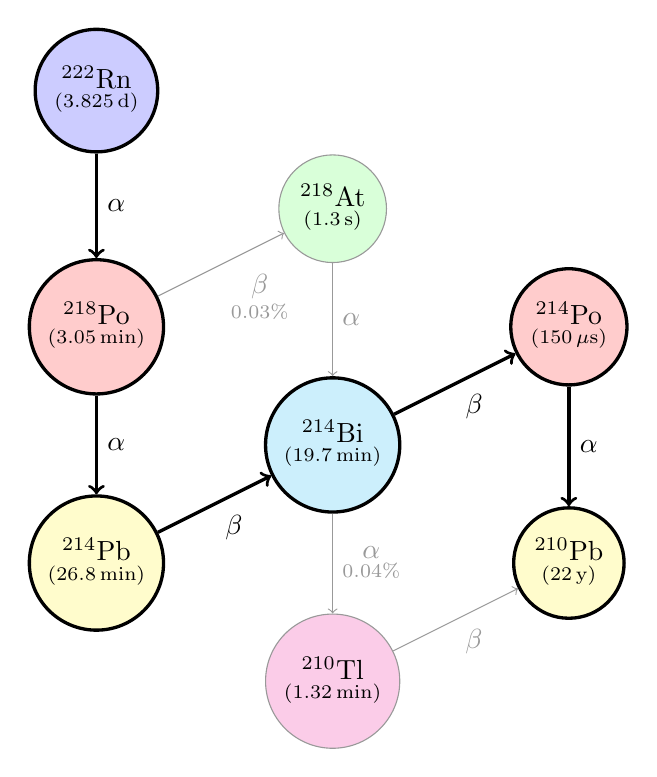
\begin{tikzpicture}
    \node (Rn222) [rn] at (0,0) { $\underset{(3.825\,\mathrm{d}) }{ { }^{222}\mathrm{Rn} } $ };
    \node (Po218) [po] at (0,-3) { $\underset{(3.05\,\mathrm{min}) }{ { }^{218}\mathrm{Po} } $ };
    \node (Pb214) [pb] at (0,-6) { $\underset{(26.8\,\mathrm{min}) }{ { }^{214}\mathrm{Pb} } $ };
    \node (Bi214) [bi] at (3,-4.5) { $\underset{(19.7\,\mathrm{min}) }{ { }^{214}\mathrm{Bi} } $ };
    \node (Po214) [po] at (6,-3) { $\underset{(150\,\mu\mathrm{s}) }{ { }^{214}\mathrm{Po} } $ };
    \node (Pb210) [pb] at (6,-6) { $\underset{(22\,\mathrm{y}) }{ { }^{210}\mathrm{Pb} } $ };
    \node (At218) [at_ig] at (3,-1.5) { $\underset{(1.3\,\mathrm{s}) }{ { }^{218}\mathrm{At} } $ };
    \node (Tl210) [tl_ig] at (3,-7.5) { $\underset{(1.32\,\mathrm{min}) }{ { }^{210}\mathrm{Tl} } $ };
    \draw[very thick, ->] (Rn222) -- node[anchor=west] {$\alpha$} (Po218);
    \draw[very thick,->] (Po218) -- node[anchor=west] {$\alpha$} (Pb214);
    \draw[very thick,->] (Pb214) -- node[anchor=north west] {$\beta$} (Bi214);
    \draw[very thick,->] (Bi214) -- node[anchor=north west] {$\beta$} (Po214);
    \draw[very thick,->] (Po214) -- node[anchor=west] {$\alpha$} (Pb210);
    \draw[black!40,->] (Po218) -- node[anchor=north west] {$\underset{0.03\%}{\beta} $} (At218);
    \draw[black!40,->] (At218) -- node[anchor=west] {$\alpha$} (Bi214);
    \draw[black!40,->] (Bi214) -- node[anchor=west] {$\underset{0.04\%}{\alpha} $} (Tl210);
    \draw[black!40,->] (Tl210) -- node[anchor=north west] {$\beta $} (Pb210);
\end{tikzpicture}
}
            \caption[Network2]%
            {{\tiny Rn-222 Decay Chain}}    
            \label{fig:UraniumChain}
        \end{subfigure}
        \hfill
        \begin{subfigure}[c]{0.49\textwidth}  
            \centering 
            \scalebox{0.5}{
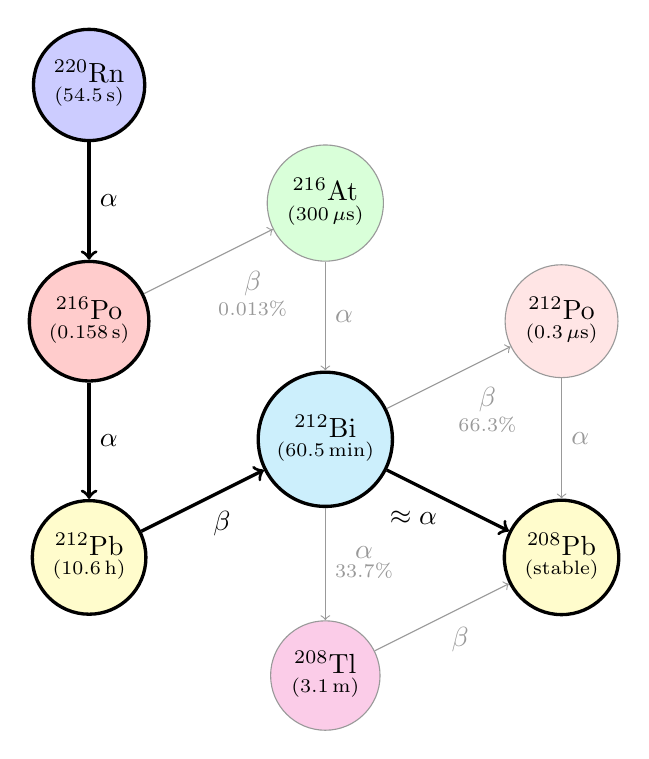
\begin{tikzpicture}
    \node (Rn220) [rn] at (0,0) { $\underset{(54.5\,\mathrm{s})}{ { }^{220}\mathrm{Rn} } $ };
    \node (Po216) [po] at (0,-3) { $\underset{(0.158\,\mathrm{s})}{ { }^{216}\mathrm{Po} } $ };
    \node (Pb212) [pb] at (0,-6) { $\underset{(10.6\,\mathrm{h})}{ { }^{212}\mathrm{Pb} } $ };
    \node (Bi212) [bi] at (3,-4.5) { $\underset{(60.5\,\mathrm{min})}{ { }^{212}\mathrm{Bi} } $ };
    \node (Po212) [po_ig] at (6,-3) { $\underset{(0.3\,\mu\mathrm{s})}{ { }^{212}\mathrm{Po} } $ };
    \node (Tl208) [tl_ig] at (3,-7.5) { $\underset{(3.1\,\mathrm{m})}{ { }^{208}\mathrm{Tl} } $ };
    \node (Pb208) [pb] at (6,-6) { $\underset{(\mathrm{stable})}{ { }^{208}\mathrm{Pb} } $ };
    \node (At216) [at_ig] at (3,-1.5) { $\underset{(300\,\mu\mathrm{s}) }{ { }^{216}\mathrm{At} } $ };
    \draw[very thick,->] (Rn220) -- node[anchor=west] {$\alpha$} (Po216);
    \draw[very thick,->] (Po216) -- node[anchor=west] {$\alpha$} (Pb212);
    \draw[very thick,->] (Pb212) -- node[anchor=north west] {$\beta$} (Bi212);
    \draw[black!40,->] (At216) -- node[anchor=west] {$\alpha$} (Bi212);
    \draw[black!40,->] (Po216) -- node[anchor=north west] {$\underset{0.013\%}{\beta}$} (At216);
    \draw[black!40,->] (Bi212) -- node[anchor=north west] {$\underset{66.3\%}{\beta}$} (Po212);
    \draw[black!40,->] (Bi212) -- node[anchor=west] {$\underset{33.7\%}\alpha$} (Tl208);
    \draw[black!40,->] (Po212) -- node[anchor=west] {$\alpha$} (Pb208);
    \draw[black!40,->] (Tl208) -- node[anchor=north west] {${\beta}$} (Pb208);
    \draw[very thick,->] (Bi212) -- node[anchor=north east] {$\approx \alpha $} (Pb208);
\end{tikzpicture}
}
            \caption[]%
            {{\tiny Rn-220 Decay Chain}}    
            \label{fig:ThoriumChain}
        \end{subfigure}
        \caption[ Decay Chains of Isotopes ]
        {\tiny Decay series for Rn-222 and Rn-220, respectively. These are based on \cite{Leighton}*{Chapter 15}. The effective linear chains are indicated in bold. } 
        \label{fig:DecayChains}
\end{figure}

\vspace*{-0.1cm}
Consider a (linearly ordered) decay chain $X_0\to X_1\to \ldots \to X_\ell$ in which the decay constant of $X_j$ is $\lambda_j$ for $j=0,1,\ldots,\ell-1$, and $X_\ell$ is stable.
We assume throughout that $\lambda_0,\lambda_1,\ldots,\lambda_{\ell-1}$ are distinct and positive.
Starting at time $0$ with a collection $N_0(0)$ atoms of $X_0$, $N_1(0)$ atoms of $X_1$, etc.,
let $N_0(t),N_1(t),\ldots,N_{\ell-1}(t)$ denote the expected number of atoms of the respective type in the given decay chain remaining at time $t$.
%Assume the $j$-th member of the chain has decay constant $\lambda_j>0$, and that $\lambda_0,\lambda_1,\ldots,\lambda_\ell$ are distinct.
When $0<j < \ell$, the number $N_j(t)$ can change over time either by the decay of an atom of type $X_j$ into one of type $X_{j+1}$ (decreasing $N_j(t)$ in the process) or by an atom of $X_{j-1}$ decaying into an atom of $X_j$ (thereby increasing $N_j(t)$). The time evolution of the ensemble is thus described by the following system of ordinary differential equations:
$$
\frac{dN_0}{dt}=-\lambda_0 N_0, \quad \frac{dN_j}{dt} = -\lambda_j N_j + \lambda_{j-1}N_{j-1} \quad (0<j < \ell).
$$
Compare with Equation (5) in \cite{Leighton}*{Chapter 15}. \\

Recall that the detector does not measure the number of atoms remaining $N_j(t)$ but instead decay counts, the expected number of which in an interval $(s_1,s_2]$ is given by a sum of expressions of the form $\int_{s_1}^{s_2}\lambda_j N_j(s)ds$. Nevertheless, it will be in our interest to solve for $N_j$ first.
The solutions of the system are provided by the \textit{Bateman Equation} \cite{Bateman} when $N_1(0)=\cdots=N_{\ell-1}(0)=0$:
$$
N_j(t) = \frac{N_0(0)}{\lambda_j}\sum_{r=0}^j\left(\prod_{q=0,q\neq r}^j \frac{\lambda_q}{\lambda_q-\lambda_r}\right)\lambda_r e^{-\lambda_r t}.
$$
Thus the number of decays by atoms of the $j$-th type in the time interval $(s_1,s_2]$ is
\begin{equation}\label{Eq:jthCount}
\int_{s_1}^{s_2} \lambda_j N_j(s)ds = N_0(0)\sum_{r=0}^j\left(\prod_{q=0,q\neq r}^j \frac{\lambda_q}{\lambda_q-\lambda_r}\right)(e^{-\lambda_r s_1}-e^{-\lambda_r s_2})
\end{equation}
Since our detector only detects alpha decays, the number of counts we expect to see in the time interval $(s_1,s_2]$ is given by
$$
\sum_{j \: \alpha\text{-decays}}\int_{s_1}^{s_2}\lambda_j N_j(s)ds.
$$

As each of these expressions shares the same independent variable $N_0(0)$, we may determine the total counts expected from this decay chain in any fixed interval as some function of only $N_0(0)$, provided we are working with a single decay chain.
For the problem under consideration, we must work with two.
The decay chains for Rn-222 and Rn-220 do not intersect, and thus the total counts from a collection of both of these isotopes of radon is the sum of the counts from the individual decay chains. In particular, the expected total number of counts in a time interval $(s_1,s_2]$ from an initial mixture of $N_{222}(0)$ atoms of Rn-222 and $N_{220}(0)$ atoms of Rn-220 is given by an expression of the form
\[ N_{222}(0)\int_{s_1}^{s_2}f_{222}(t)dt+N_{220}(0)\int_{s_1}^{s_2}f_{220}(t)dt, \]
where $f_{222}$ and $f_{220}$ are functions derived from \eqref{Eq:jthCount}.
This indicates that linear regression will provide an effective means of extracting the coefficients to determine the quantities of Rn-222 and Rn-220 present in a given sample.\\

Using the expected number of decays and the observed counts, we use a linear regression model to estimate our initial amount of each isotope. Letting $P$ be the total number of sampling periods, we fit the model:
    \begin{align*}
        y_i &= N_{222}(0) {x_{222}}_i + N_{220}(0) {x_{220}}_i + \epsilon_i
    \end{align*}
where $y_i$ is the number of alpha particle decays observed in the time interval $(s_{i-1}, s_i]$, ${x_{222}}_i = \int_{s_{i-1}}^{s_{i}}f_{222}(t)dt$, ${x_{220}}_i=\int_{s_{i-1}}^{s_i}f_{220}(t)dt$, $s_i$ denotes the end of sample period $i$, for $1\leq i \leq P$, and $s_0$ denotes the beginning of sample period $1$. Note that the errors $\epsilon_1,\ldots,\epsilon_P$ are random but not independent of one another.\\
%To account for the intake time of the sniffer, we consider an offset in these equations that change the inputs by the amount of time it takes for the sniffer to fill the chamber (in our case this is $90$ seconds). The output, $y_i$, is the number of alpha particle decays counted in the previous sampling period, and where $\epsilon_i$ is a random variable. Using this model, we solve for the coefficients $\hat{N}_{222}(0)$ and $\hat{N}_{220}(0)$ which give us an estimated total number of atoms at the start time of the experiment for each nuclide.\\
\vspace*{-0.5cm}
\subsection{Simulating Experimental Values}\label{SS:SimulatingExperimentalValues}

In order to design the optimal sampling scheme, we must be able to evaluate the effectiveness of the linear regression model for any particular scheme. Determining this analytically is not straightforward, as the counts in any particular period are random and depend on the state underlying the counts in the previous period, as well as the length of each period. Even for a single particle, the time at which it decays into any other particle in the chain is the sum of random variables from several exponential distributions with different parameters. Therefore, we elected to evaluate the effectiveness of a scheme over test data, which we generated. We also narrowed the scope of sampling schemes under consideration to schemes where counts are reported at fixed times, over a fixed duration of time, where the contents of the cell are held constant over that duration. This sampling scheme does also require that we consider a time offset in order to account for the time it takes to fill the chamber, or else we would underestimate the Rn-220. Phrased in terms of the previous section, $s_i = T_s \cdot i + T_f$ for $0\leq i\leq P$, where $T_s$ is time of the sampling period and $T_f$ is the time taken to fill the chamber.\\

This differs from the typical method used by radon mitigators in the field, which is continuous sampling of some number of environments, interspersed with flushing periods. However, based on our early results, we do not believe that this is a viable scheme to determine the relative amounts of Rn-220 and Rn-222, as the half-lives are too different and variations during pumping are not well understood. This change in procedure is a reasonable compromise, as in most circumstances knowing the Rn-220 concentration isn't necessary, and in those situations where it is the sampling scheme we propose is acceptable. \\

Generating test data for a sampling scheme of this type is relatively straightforward, but as the random processes involved are complicated, the best method we were able to come up with is not particularly efficient, having time complexity of $O(N\cdot \ell)$, where $N$ is the number of particles in the chain at time $t=0$ and $\ell$ is the length of the chain. We assume that at time $t=0$, for a given decay chain, that only the substance at the head of the chain is present. Then, for each particle of that substance, we sample the \textit{particle lifetimes}, which is the time that particle will take to decay from each substance in the decay chain to the next substance. Then the time at which that particle decays into each substance is the cumulative sum of the particle lifetimes up to that point. Using these decay times for the particles, we can then count how many alpha decays occur in each sampling period, which gives us the observed count for that sampling period.\\

\subsection{Model Visualization}\label{SS:ModelVisualization}

To demonstrate the relationship between the expected counts and the generated count data, we graph the expected count rate and a corresponding sample run for a series of concentration levels in Figure \ref{fig: SampleRuns}. Homeowners are advised to take action if the radon activity is greater than 4 pCi/L in air \cite{EPA}, sub-slab measurements can be on the order of $100$ pCi/L, and the largest value that Environmental Instruments Canada has reported to us was around $8000$ pCi/L. By showing these values, we can see the amount of variation implicit to this problem, and note that higher activities make it much easier to determine the amounts of Rn-222 and Rn-220.
%It should be noted that $4$ pCi/L of Rn-220 corresponds to about 12 atoms per litre.
\begin{figure}[h]
        \centering
        \begin{subfigure}[c]{\textwidth}
            \centering
            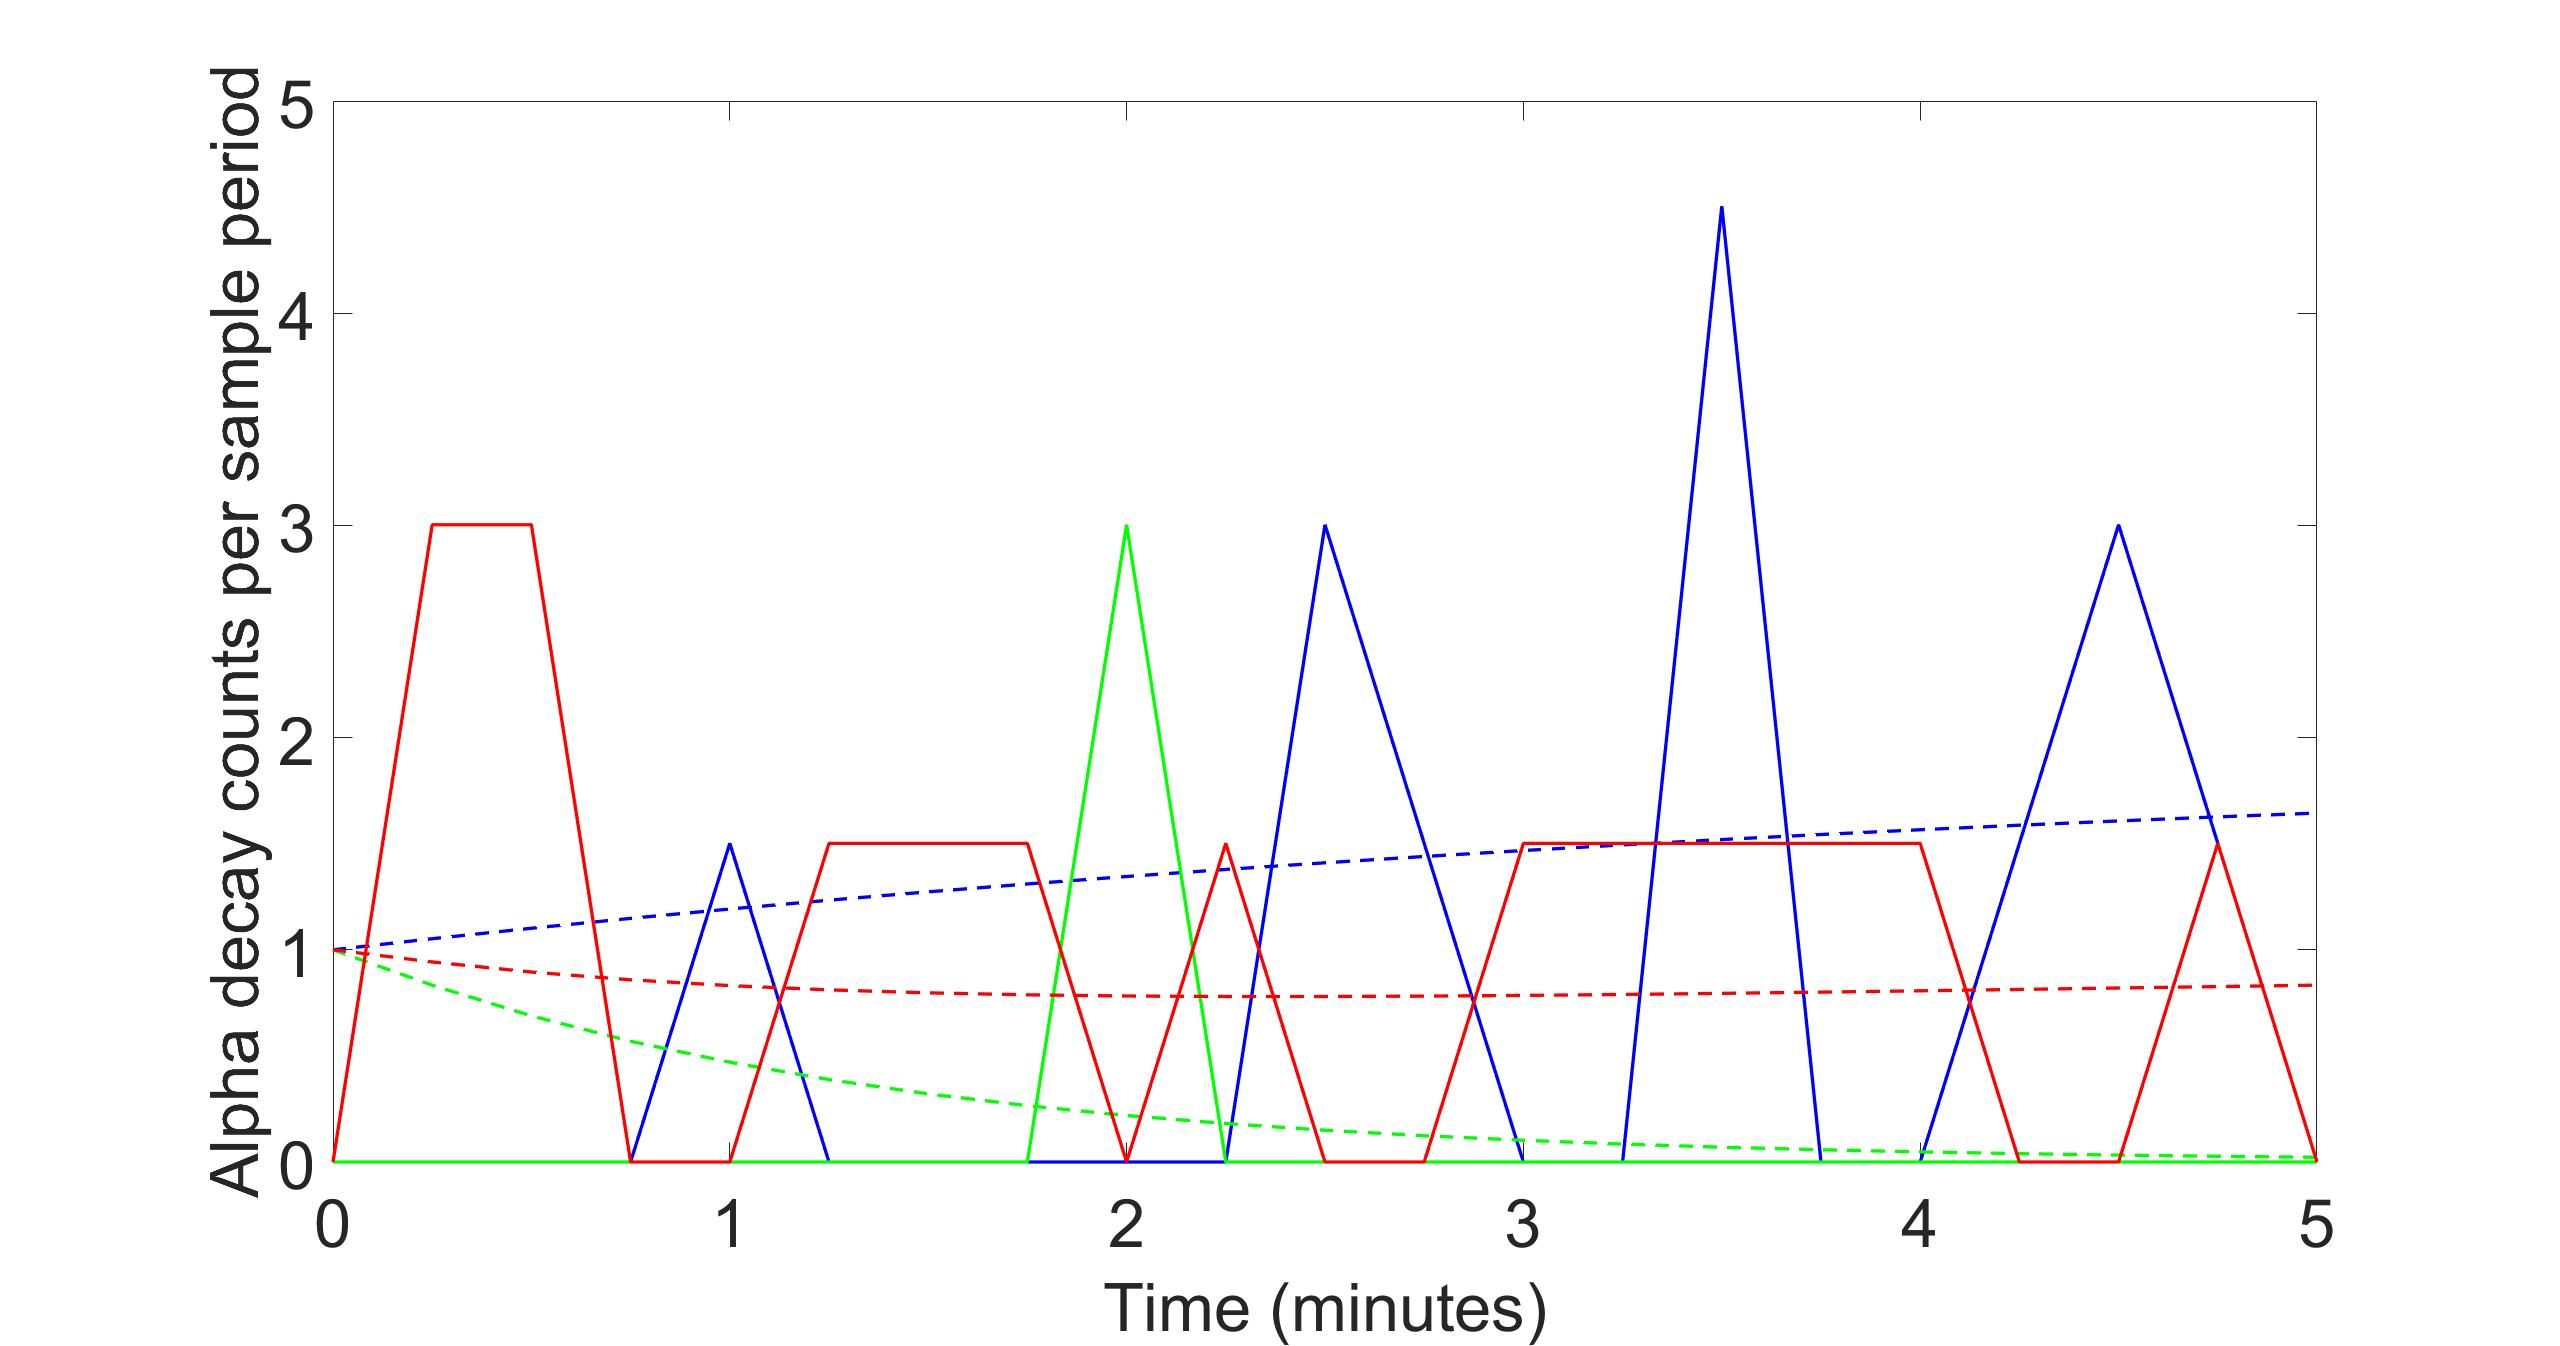
\includegraphics[scale=0.0825]{images/new_4pcpl.jpg}
            \caption[Network2]%
            {{\tiny Activity level of 4 pCi/L}}    
            \label{fig:LowActivitySample}
        \end{subfigure}
\end{figure}
\begin{figure}[h]\ContinuedFloat
	\centering
        %\hfill
        \begin{subfigure}[c]{0.475\textwidth}  
            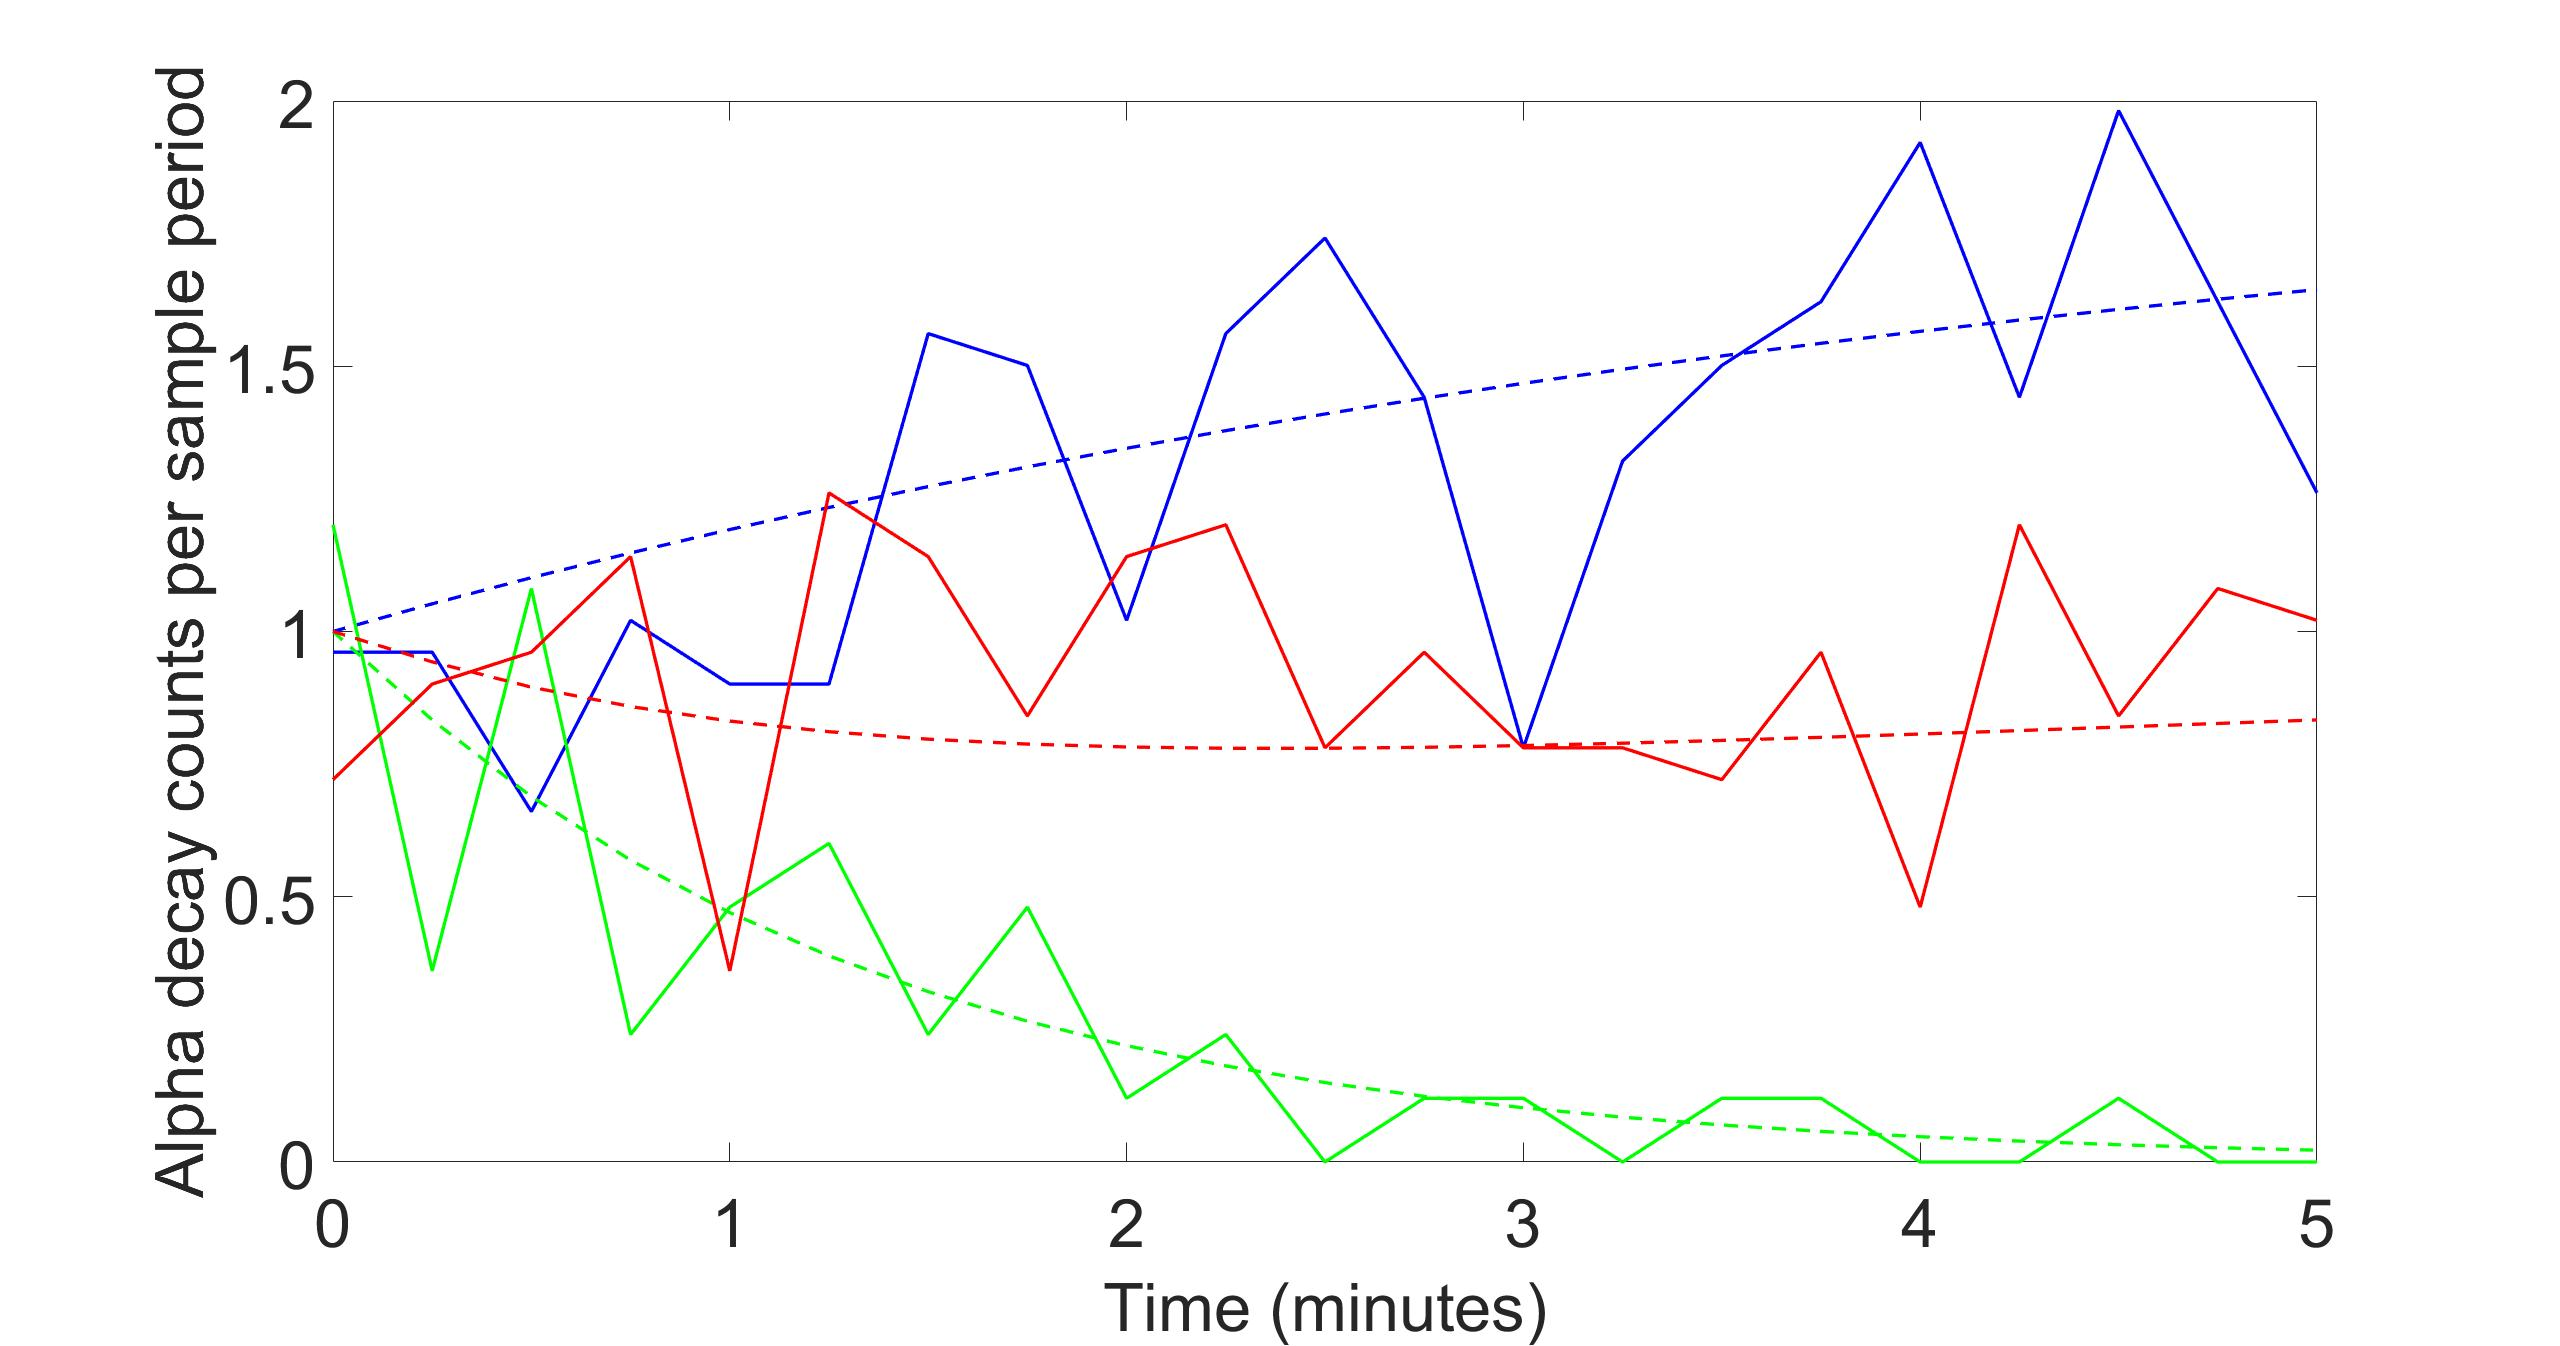
\includegraphics[scale=0.0825]{images/new_100pcpl.jpg}
            \caption[]%
            {{\tiny Activity level of 100 pCi/L}}    
            \label{fig:MediumActivitySample}
        \end{subfigure}
        \begin{subfigure}[c]{0.475\textwidth}   
            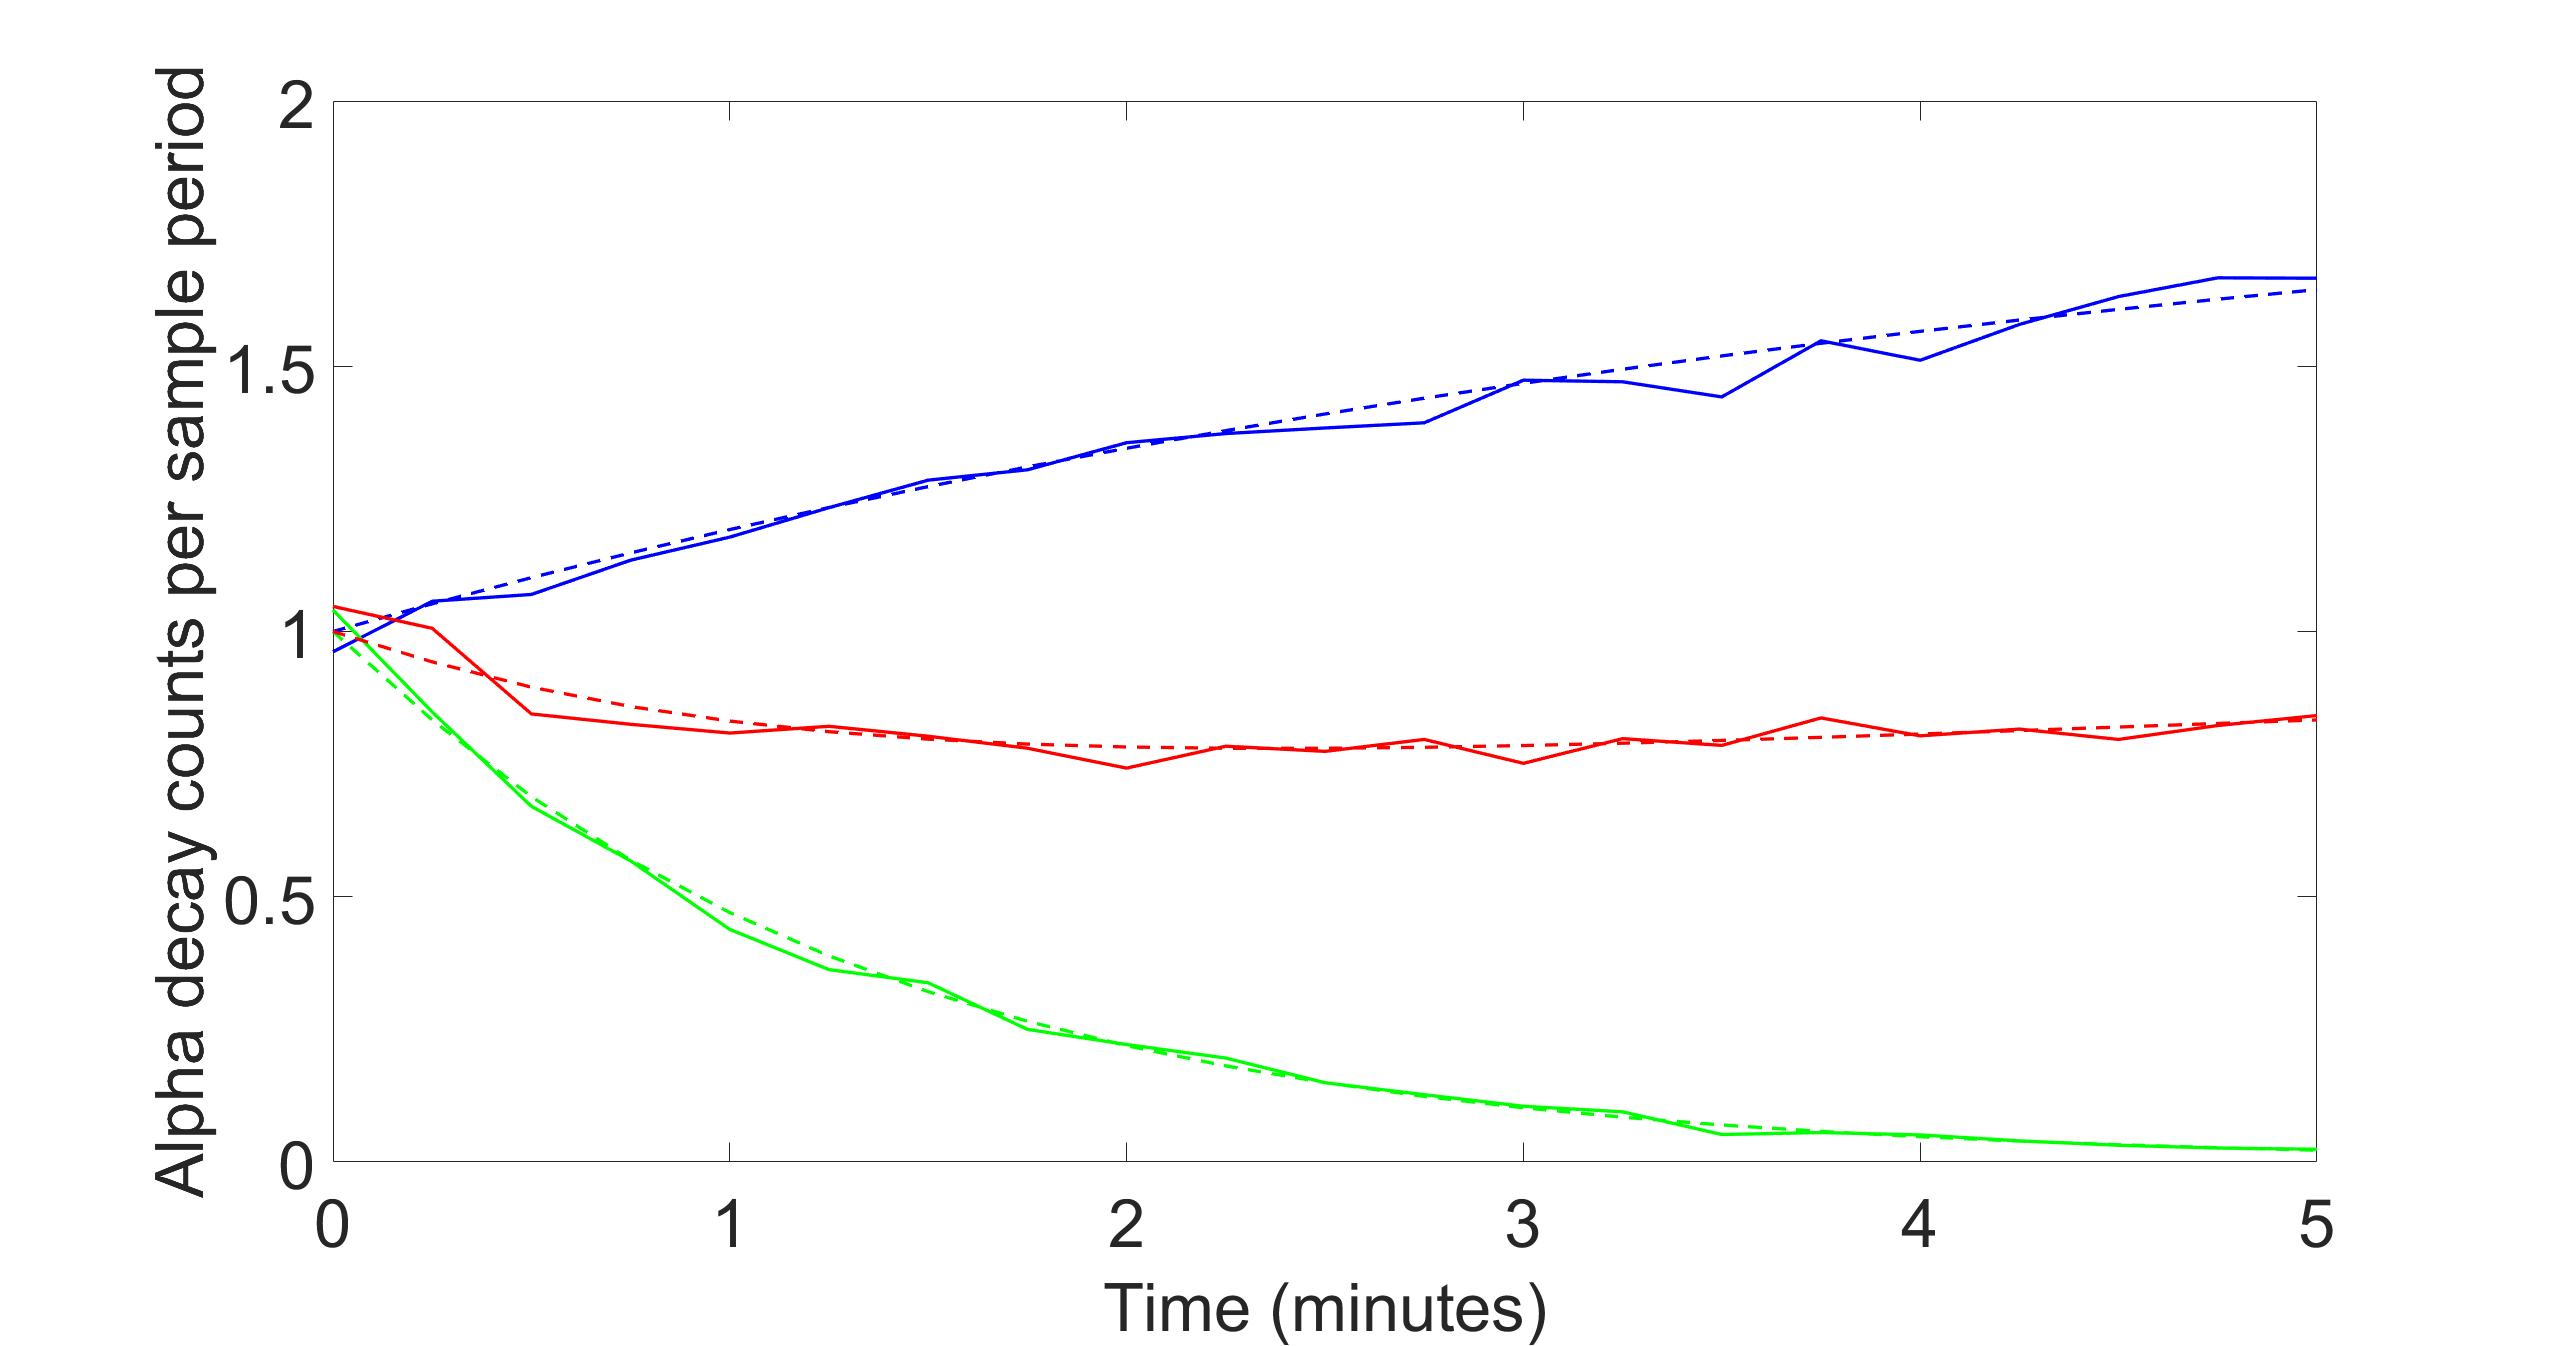
\includegraphics[scale=0.0825]{images/new_8000pcpl.jpg}
            \caption[]%
            {{\tiny Activity level of 8000 pCi/L}}    
            \label{fig:HighActivitySample}
        \end{subfigure}
        \caption[ The average and standard deviation of critical parameters ]
        {\tiny Sample runs and expected values for various mixtures of Radon isotopes (blue: pure Rn-222, red: Rn-222/Rn-220 mixture, green: pure Rn-220; dashed: expected counts, continuous: observed counts) } 
        \label{fig: SampleRuns}
\end{figure}

\vspace*{-0.3cm}
\section{Parameter Estimation}\label{S:ParameterEstimation}
\subsection{Grid Search}\label{SS:GridSearch}
To find the sampling time and sampling period which minimize the variance in the estimates, we run a grid search that calculates multiple regressions on a fixed set of concentrations. Running a new sample set of decays for each regression is done to avoid over-fitting the model to a training set of data. From here, we calculate the mean and standard deviation of the estimated coefficients for various combinations of the sampling time and period to find appropriate values, attempting to minimize both the error relative to the true concentration, and the standard deviation in the estimates. With any sampling time below $90$ seconds, we were not able to see a separation between the Rn-222 and Rn-220.
%so our model was highly inaccurate.
When we sample for longer, our estimates start to level off in accuracy and increased time is no longer needed. From figure \ref{fig:Gridsearch} we see that the standard deviations level off at approximately $5$ minutes duration and are mostly independent of sampling period. \\%Given this information we will select the minimum required time for the sampling time at $5$ minutes and a sampling period of $3$ seconds.  \\

For each potential sampling time and period, the actual model with which estimations can be made takes the form of the $2\times P$ matrix described by the left pseudo-inverse of $X$, $(X^TX)^{-1}X^T$, where the $P\times 2$ matrix $X=\begin{bmatrix} {x_{222}} & {x_{220}}\end{bmatrix}$ is formed using the values for ${x_{222}}$ and ${x_{220}}$ determined using the grid search, and when given a sample vector $y$, the estimated amounts $\hat{N}_{222}$ and $\hat{N}_{220}$ are determined by
\begin{align*}
    \begin{bmatrix}
    \hat{N}_{222}\\
    \hat{N}_{220}
    \end{bmatrix} = (X^TX)^{-1}X^T y
\end{align*}
\begin{figure}[h]
\centering
        \begin{subfigure}[c]{\textwidth}
            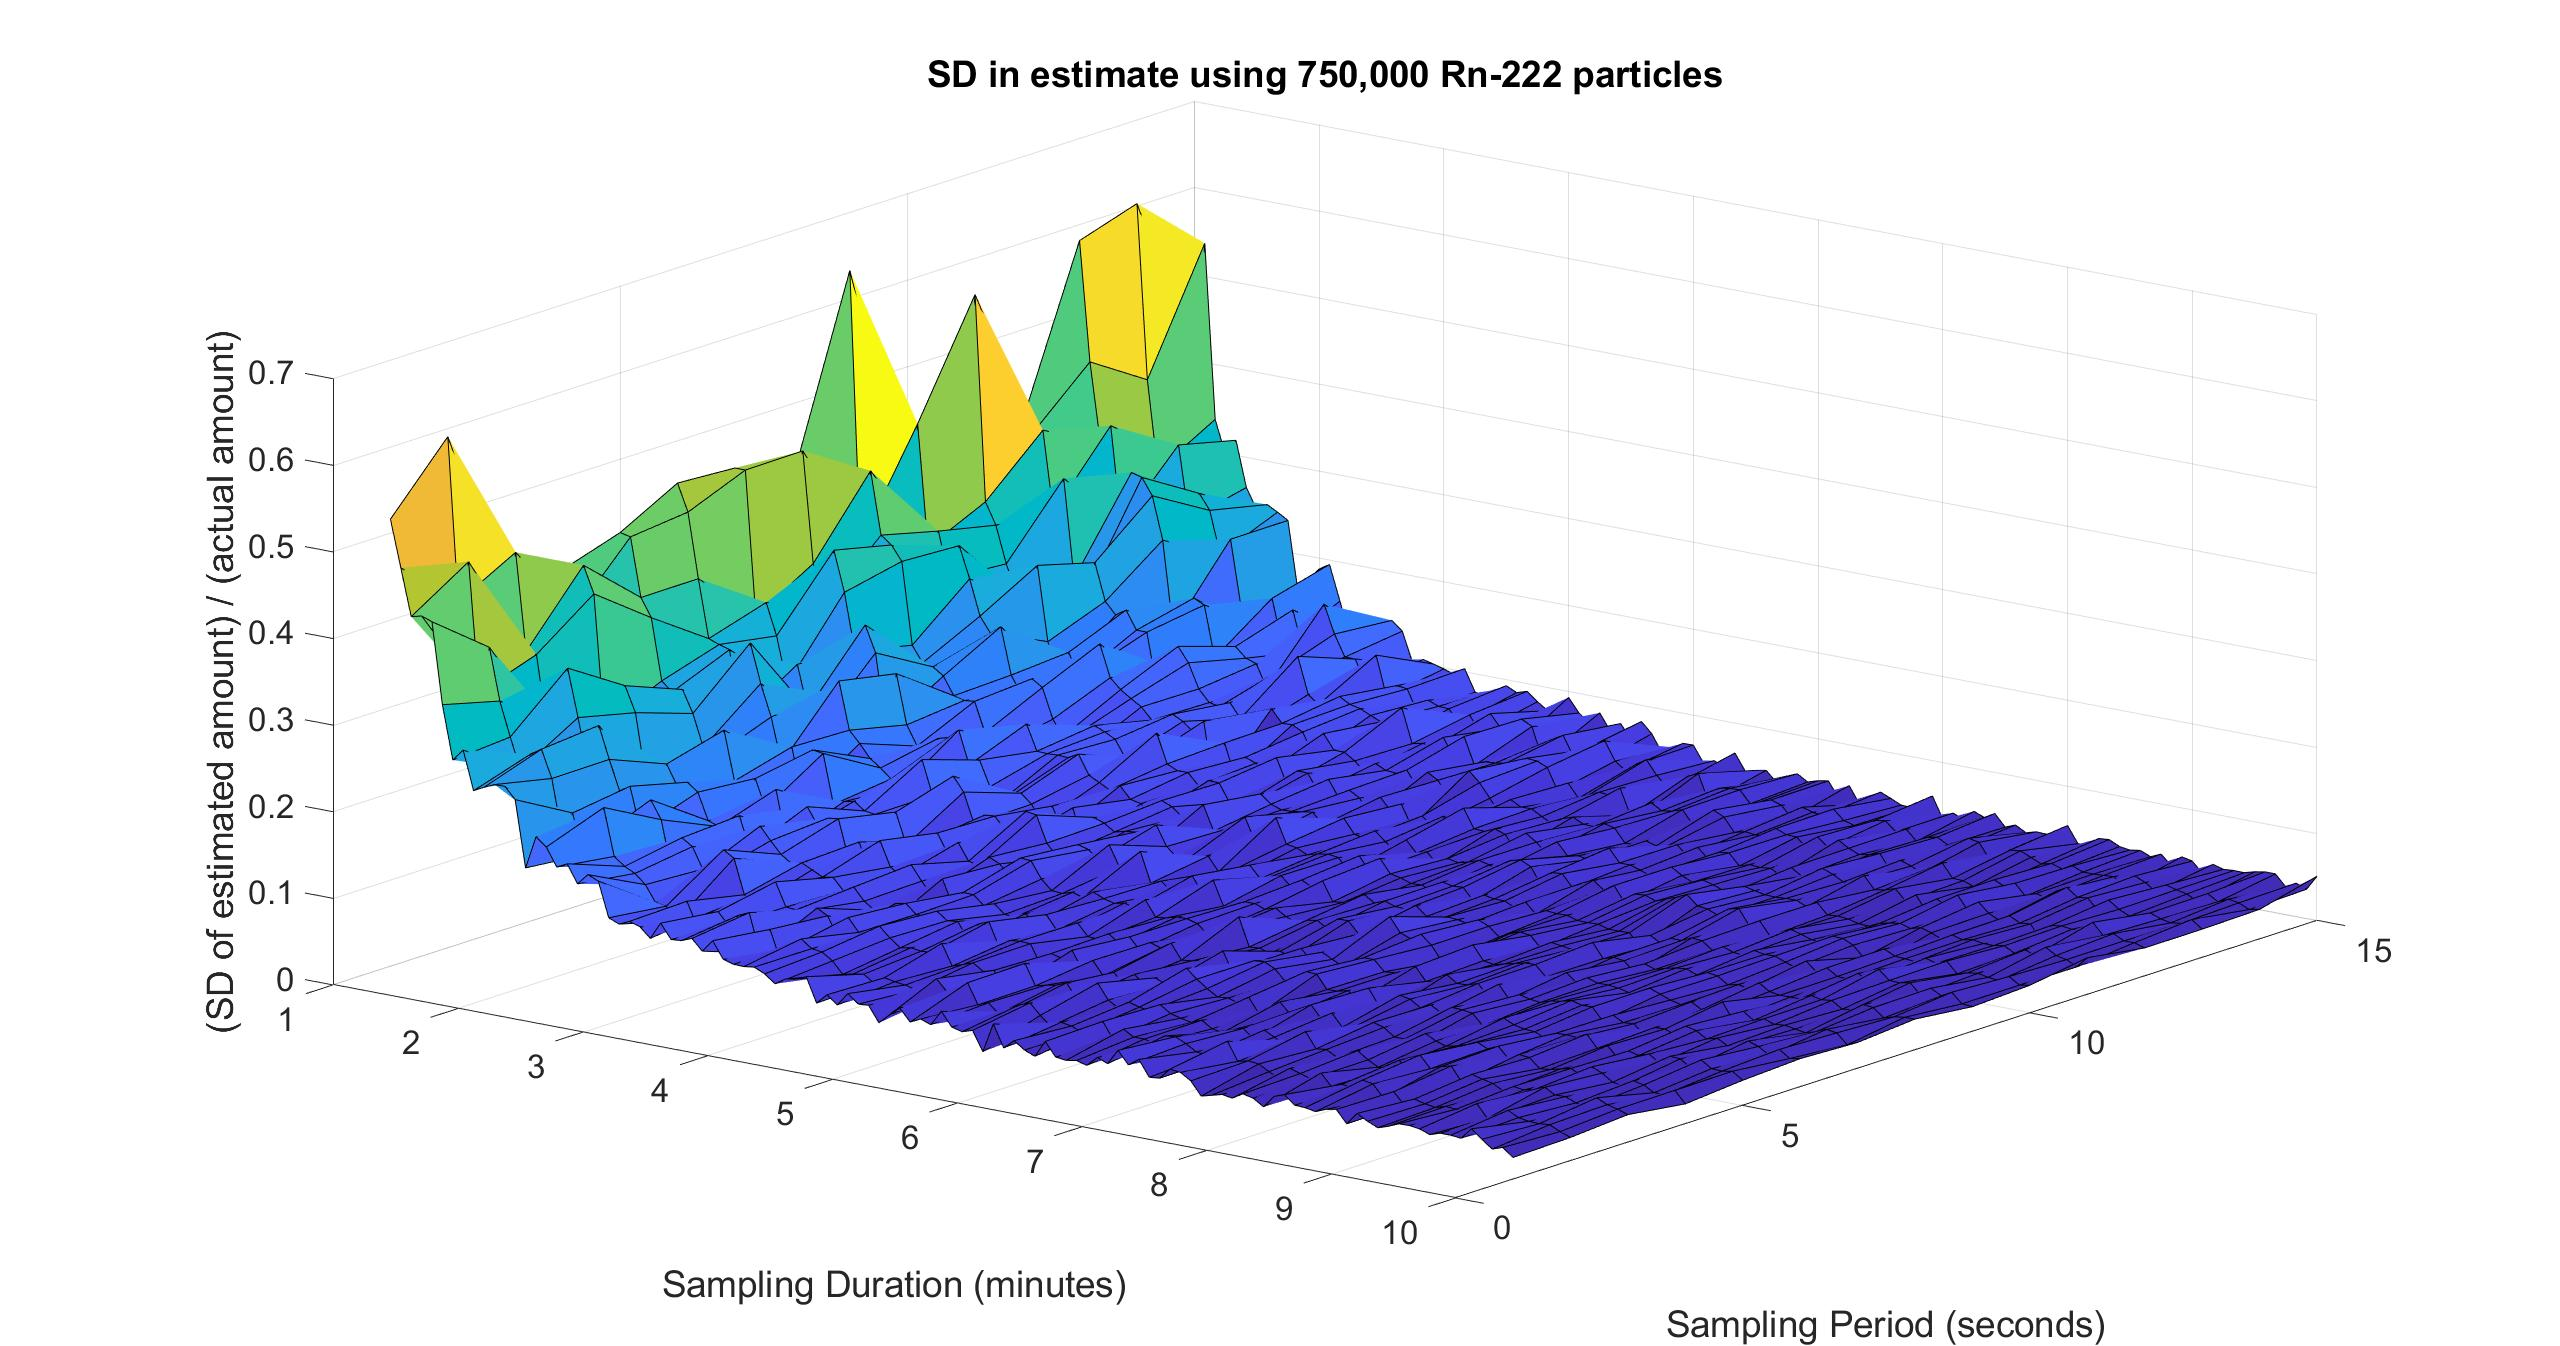
\includegraphics[scale=0.14]{images/std_rn222_gridsearch.jpg}
            \caption[Network2]%
            {{\tiny Standard deviation of $25$ different linear regression estimates for radon}}    
            \label{fig:RadonGridsearch}
        \end{subfigure}
        %\hfill
        
\end{figure}
\begin{figure}[h]\ContinuedFloat
\centering
        \begin{subfigure}[c]{\textwidth}  
            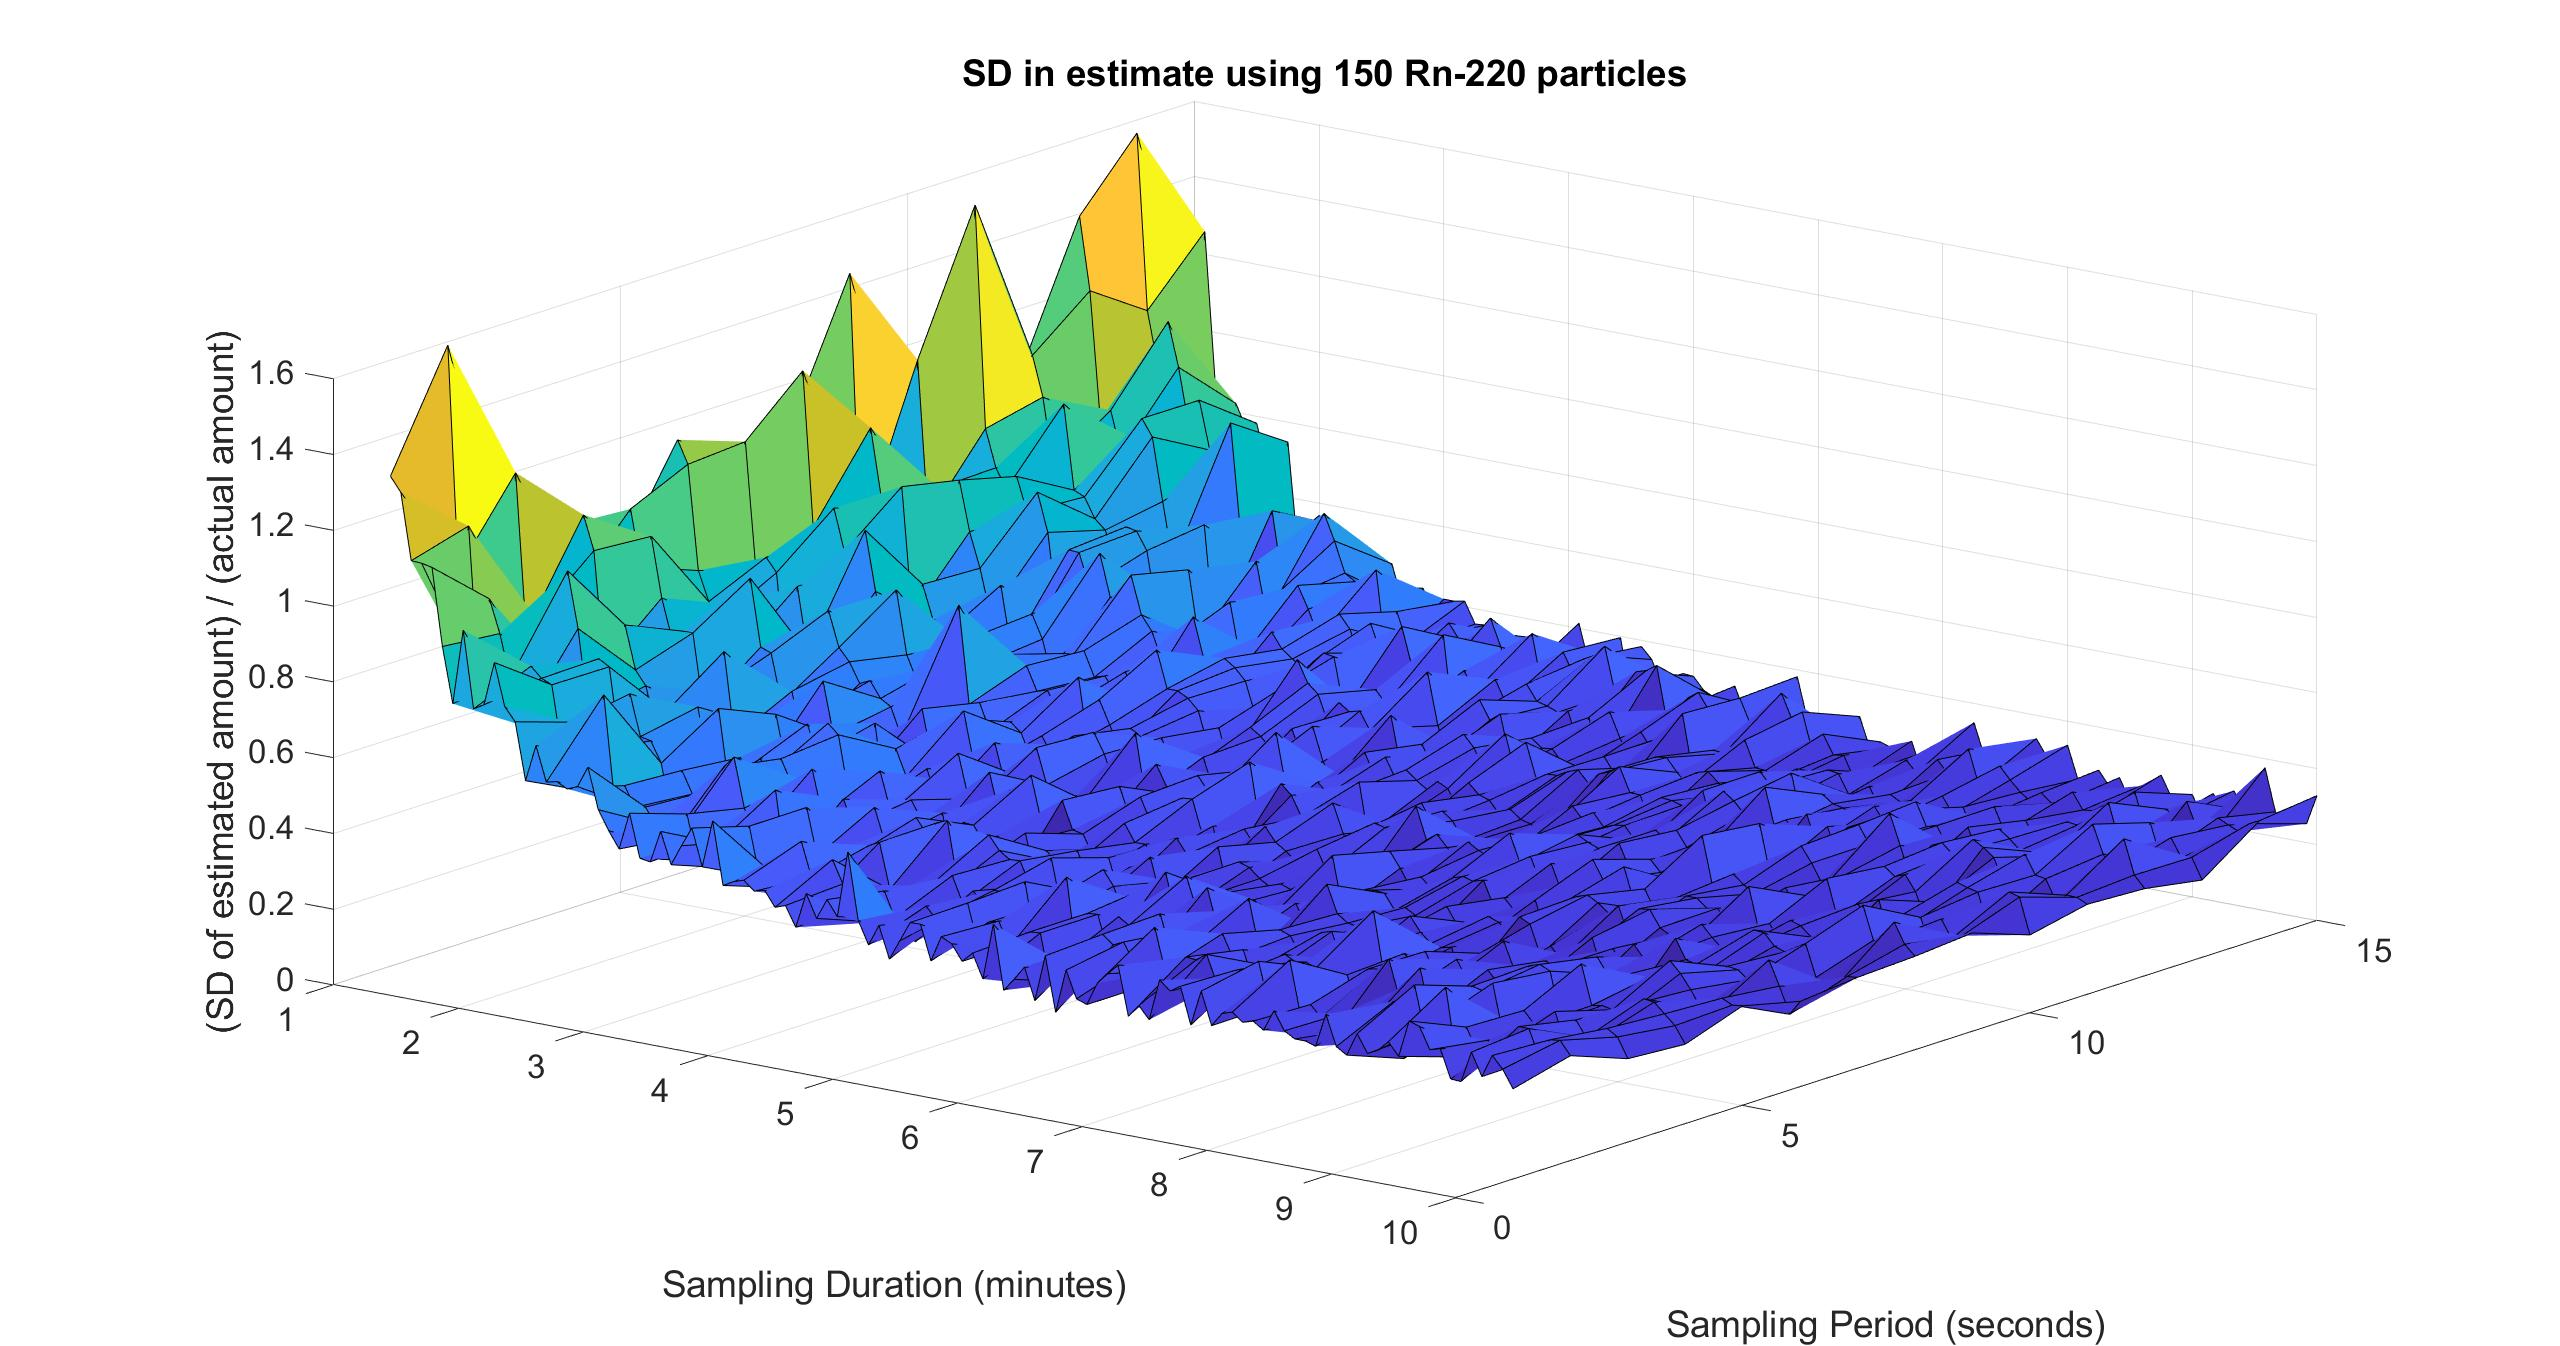
\includegraphics[scale=0.14]{images/std_rn220_gridsearch.jpg}
            \caption[]%
            {{\tiny Standard deviation of $25$ different linear regression estimates for thoron}}    
            \label{fig:ThoronGridsearch}
        \end{subfigure}
        \caption[ The average and standard deviation of critical parameters ]
        {\tiny Standard deviation in estimated values over varied sampling parameters} 
        \label{fig:Gridsearch}
\end{figure}


\subsection{Results}\label{SS:Results}

After tuning our sampling parameters, we requested and received data on different radon and thoron sources from EIC. Using this data, we fit our linear regression model and solve for our initial concentrations of Rn-222 and Rn-220. Using those estimates rounded up to the next whole number, we then solve for what the expected number of alpha decays would be over our $5$ minute interval and generate test data for the same amount of each nuclide. The following graphs highlight the accuracy of our model.\\

From figures \ref{fig:RealWorldTests} (a)-(d), we see that our model can predict the radon levels for a typical basement as well as the extreme cases where we are measuring high concentrations of Rn-220. These measurements where done all in the same day so the progeny of the previous test would be included in each subsequent test, therefore causing more error into our model. Although our predictions appear to be fairly accurate, they rely on the assumption that our radon sniffing chamber is empty. This progeny remaining in the sniffer will cause our model to overestimate the true values and a correction to the alpha decay count could increase the effectiveness of our model.
\begin{figure}[h]
        \centering
        \begin{subfigure}[c]{0.475\textwidth}
            \centering
            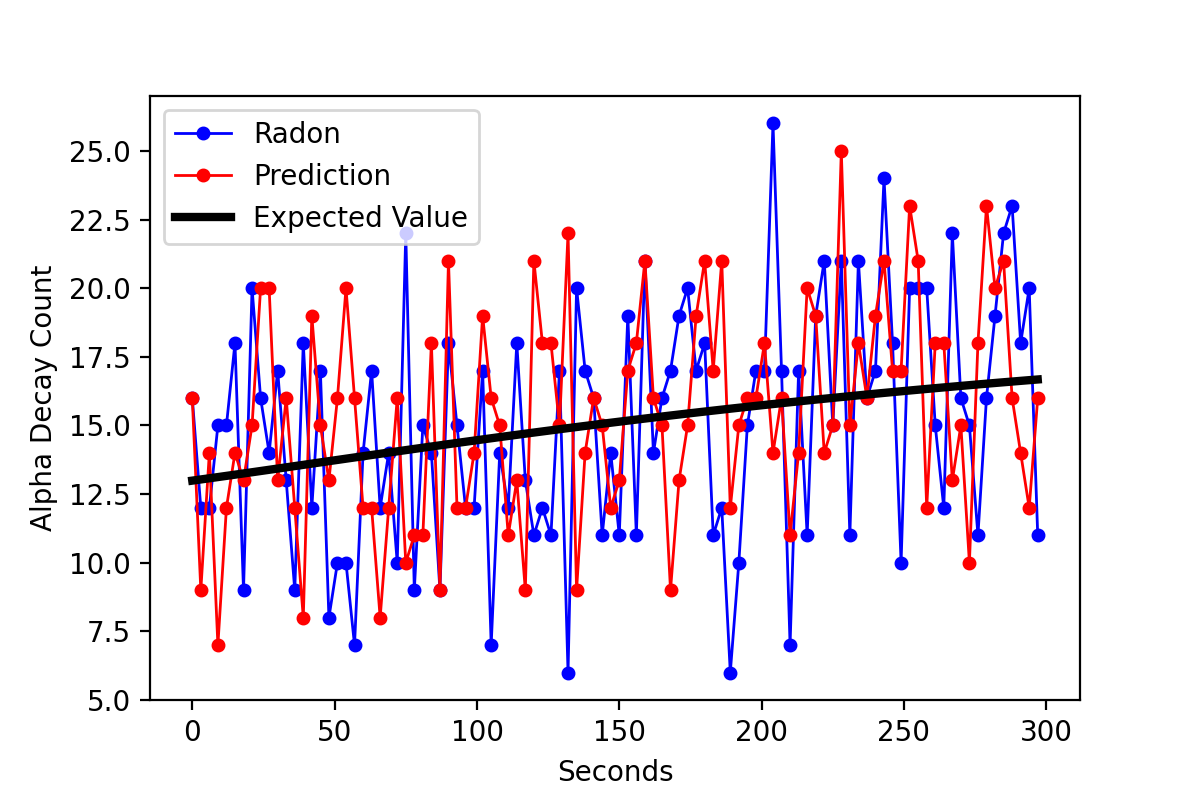
\includegraphics[scale=0.425]{images/Radon_Trial1.png}
            \caption[Network2]%
            {{\tiny First Radon Sample}}    
            \label{fig:RadonTrial1}
        \end{subfigure}
        %\hfill
        \begin{subfigure}[c]{0.475\textwidth}  
            \centering 
            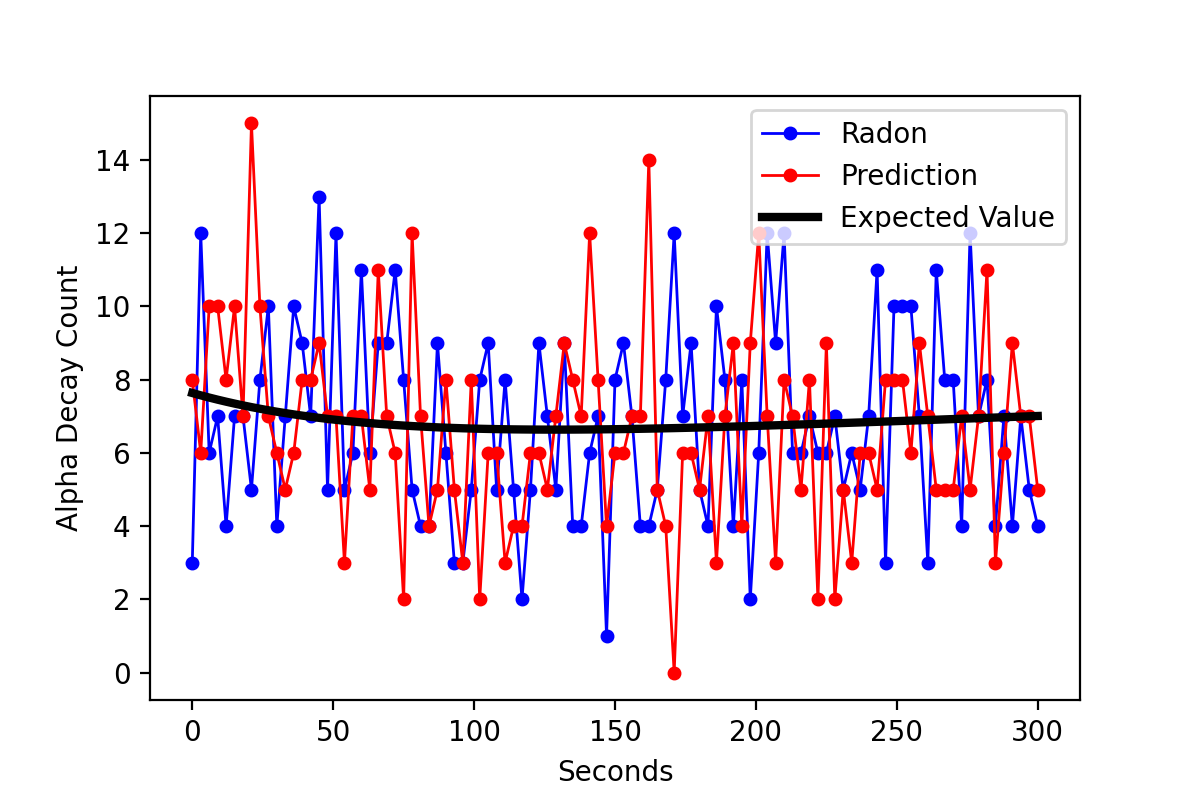
\includegraphics[scale=0.425]{images/Radon_Trial2.png}
            \caption[]%
            {{\tiny Second Radon Sample}}    
            \label{fig:RadonTrial2}
        \end{subfigure}
\end{figure}
\vspace*{-0.45cm}
\begin{figure}[h]\ContinuedFloat
        \centering
        %\vskip\baselineskip
        \begin{subfigure}[c]{0.475\textwidth}   
            \centering 
            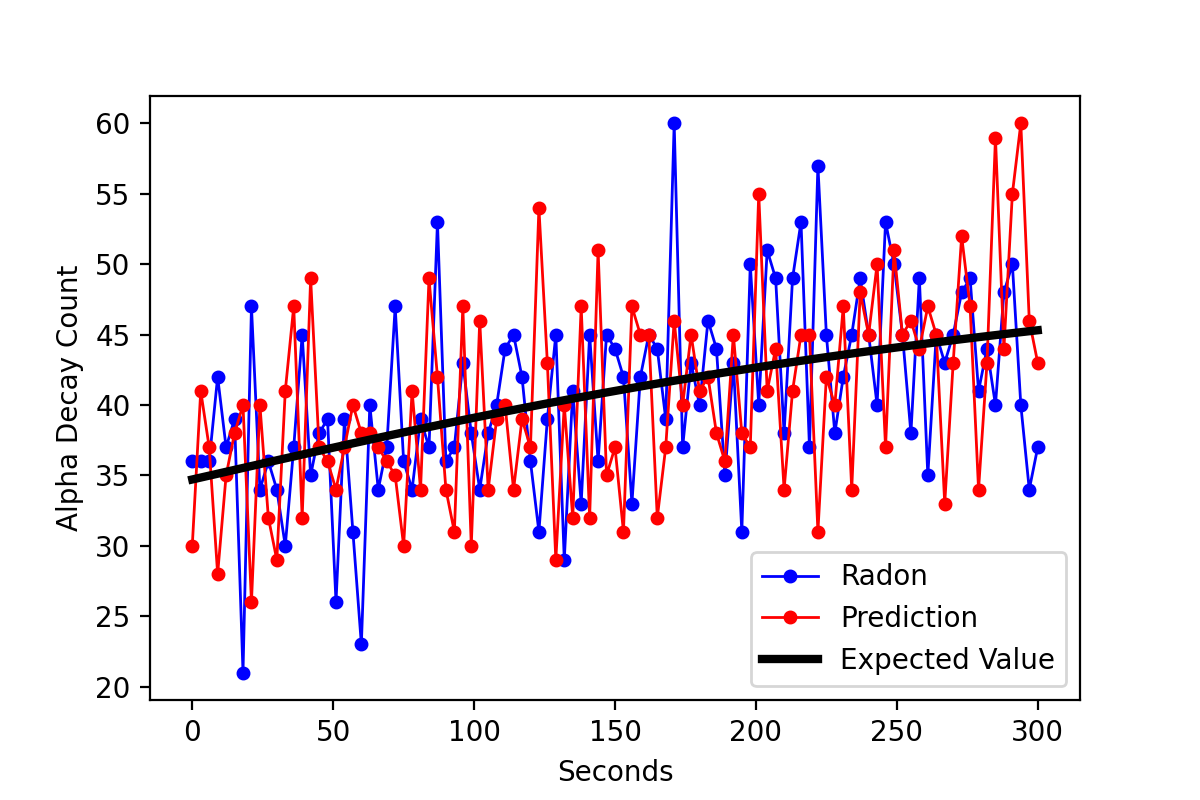
\includegraphics[scale=0.425]{images/Radon_Trial3.png}
            \caption[]%
            {{\tiny Third Radon Sample}}    
            \label{fig:RadonTrial3}
        \end{subfigure}
        %\hfill
        \begin{subfigure}[c]{0.475\textwidth}   
            \centering 
            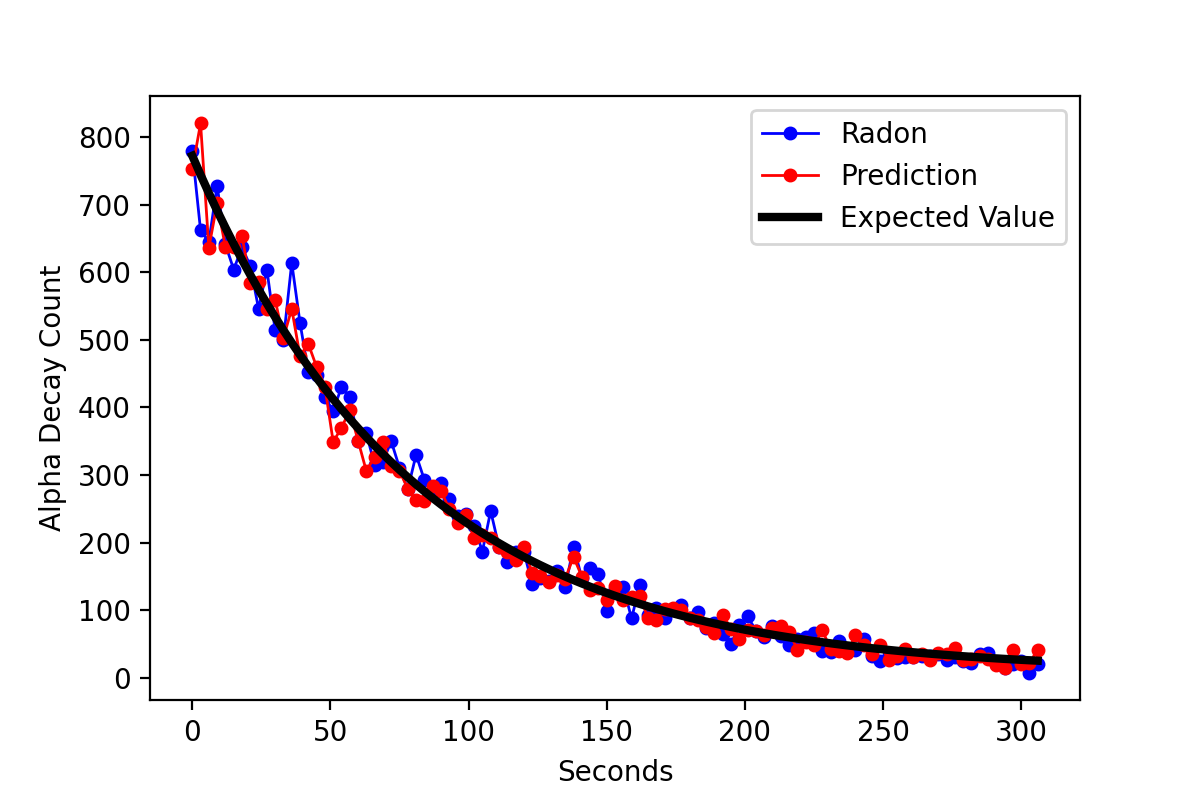
\includegraphics[scale=0.425]{images/Thoron_Trial1.png}
            \caption[]%
            {{\tiny Thoron Sample}}    
            \label{fig:ThoronTrial}
        \end{subfigure}
        \caption[ The average and standard deviation of critical parameters ]
        {\tiny Observed and Predicted Values of Radon Samples} 
        \label{fig:RealWorldTests}
\end{figure}
\subsection{How to use the results}\label{SS:HowToUse}
Overall, based on the efficacy of our model on these sample data, and in consultation with Environmental Instruments Canada, we have selected a sampling period of $3$ seconds, over a total duration of $5$ minutes. The particular sampling schedule is as follows:
\begin{enumerate}
    \item Flush the cell for ~ $90$ seconds (this is probably an overestimation of the time required).
    \item Pump air from the spot to be sampled into the cell for $90$ seconds (this is also probably an overestimation of the time required).
    \item Stop the pump, to let the sample be measured. Counting for this sequence should begin here.
    \item Let the sample sit for $5$ minutes, reporting counts every $3$ seconds.
    \item Take the reported counts as a $100$ element column vector. 
    \item Multiply this vector by the $2\times 100$ matrix $(X^TX)^{-1}X^T$, where $X$ is the $100\times 2$ matrix $\begin{bmatrix} x_{222} & {x_{220}} \end{bmatrix}$, using $x_{222}$ and ${x_{220}}$ determined from the solutions to the Bateman equations over the intervals (Python code to generate each of $x_{222}$, ${x_{220}}$, $X$, and $(X^TX)^{-1}X^T$ is available on the project's GitHub repository)\cite{Github}. Note also that:
    \begin{itemize}
        \item the values $x_{222}$ and ${x_{220}}$ also need to account for the delay of pumping (in this particular setup, this can be done simply by computing the solutions for the first $130$ intervals, and ignoring the first $30$); and
        \item this matrix is constant for a given sampling schedule, and does not need to be recomputed each time. 
    \end{itemize}
    \item This gives the $2$-element column vector $\begin{bmatrix}\hat{N}_{220} & \hat{N}_{222}\end{bmatrix}^T$, which estimates the number of particles of each isotope that were in the chamber at the beginning of pumping (under the various assumptions of the underlying physics within the chamber). 
    \item Assuming that $\lambda$ is given in $s^{-1}$, the absolute activity of each can then be determined in Bq as $\lambda\hat{N}$, and the volumetric activity can then be determined using the volume of the scintillation cell.
\end{enumerate}
\vspace*{-0.5cm}
\section{Further Research}
Further analysis could be done on the model to consider various constraints. A non-negative least squares regression would constrain the estimated amounts of each isotope to be positive.  In our experimentation with this model, it tended to remove one of the covariates and predict either pure Rn-222 or pure Rn-220. Other regression methods such as Poisson regression or negative binomial regression could be considered to account for the discrete output, however when we compared our results to a normal Q-Q plot, the model fairly accurately followed a normal distribution, so these other methods may be unnecessary. Adding a correction term to the alpha decay count to account for the progeny left in the chamber could also increase the accuracy of the model. \\

To speed up the optimization, instead of considering a new dataset for each regression we could consider a fixed number of data sets for training. This would allow us to reduce the computation time, allowing us to check a finer grid of parameters. \\

Grid search is not a particularly effective method of finding the optimal configuration, so another optimization algorithm may be useful. The reason this was not done here is that the optimization variables include the sampling period and duration, and as these determine not only the distributions of the random variables under consideration, but also the constants used in any optimization model, this makes creating an analytic model which can be given to a solver very difficult. Stochastic methods using randomly generated data are better suited to this task, but still encounter issues.\\

Developing a model which determines the amount of each nuclide over time when the chamber is being filled from a source of particular concentration may allow this model to use additional data from the fill period or the purge period, and may also allow it to be extended to continuous sampling.\\

The relative error in the amount of Rn-220 is quite high. To achieve activity commensurate with that of Rn-222, one requires much lower concentrations of Rn-220, so the relative variability in counts per period is much higher. There may be heuristic methods of determining whether there is Rn-220 that could supplement this model, which may reduce the error caused by this, but we do not consider them here.\\

Due to the aforementioned inefficiency, the method we used for generating random data is only viable for relatively small numbers of particles ($N \ll 10,000,000$). For numbers of particles greater than this, another method should be developed. We sidestepped this issue by running trials in parallel, but this solution will not work for significantly larger numbers of particles.


\section{Conclusion}
Using the $90$ second procedure of continuous sniffing, we were able to measure how much Rn-222 is in our measurements. However, using this same sample scheme, we were unable to consistently differentiate between data obtained by measuring pure Rn-222 and that obtained from a mixture of Rn-222 and Rn-220. As such, we evaluated different sampling times and periods in which to most accurately estimate the quantity of each radon isotope. With this new sampling scheme of $3$ second samples counted over a time of $5$ minutes, we developed an algorithm by which the amount of Rn-220 in a sub-slab measurement of radon isotopes can be estimated through a linear regression model. In tandem with existing methods, this can be used to assist radon mitigators in making mitigation decisions by ensuring they have as much information as possible about the situation, without drastically increasing the time for each test.

% Thank people here. Replace by the plural ``Acknowledgements'' if thanking multiple people.
\section*{Acknowledgements}
We wish to thank Kai Kaletsch from Environmental Instruments Canada for assisting us in his role as an industry mentor, and for providing an interesting challenge to work on. We also wish to thank the Pacific Institute for Mathematical Sciences (PIMS) for running the $\textit{Math}^\textit{Industry}$ workshop, and the organizers within PIMS who put in a great deal of effort to make it happen.

\newpage

\begin{thebibliography}{99}



\bibitem{LungCancerCanada} Lung Cancer Canada, "Radon", \url{https://www.lungcancercanada.ca/Lung-Cancer/Radon.aspx#:~:text=Health\%20Canada\%20recently\%20increased\%20its,deaths\%20globally\%20are\%20radon\%20induced.}

\bibitem{EIC} Environmental Instruments Canada, "CT007-R Radon Sniffer",
\url{https://radonsniffer.com/}

\bibitem{NuDat} Brookhaven National Laboratory, "NuDat 2", \url{https://www.nndc.bnl.gov/nudat2/}

\bibitem{Leighton} R. B. Leighton, \textit{Principles of Modern Physics}, McGraw-Hill, New York, 1959. 

\bibitem{Bateman} H. Bateman, \textit{The solution of a system of differential equations occurring in the theory of radioactive transformations}. Proc. Cambridge Philos. Soc, Vol. 15, No. pt V (1910) pp. 423–427.

\bibitem{EPA} US Environmental Protection Agency, "Health Risk of Radon", \url{https://www.epa.gov/radon/health-risk-radon}

\bibitem{Github}
\url{https://github.com/StephenStyles/Radon}

\end{thebibliography}


\end{document}


